% -*- TeX:SI -*- slovene sub-mode for spell check
%%%%%%%%%%%%%%%%%%%%%%%%%%%%%%%%%%%%%%%%%%%%%%%%%%%%%%%%%%%%%%%%%%%%%%%%%%%%%%%%%%%%%%%%%%%%%%%%%%%%%%%%%%%%%%%%%%%%%%%%
% LaTeX predloga za zaključna dela Univerza v Ljubljani, Fakulteta za elektrotehniko Zbral in uredil: Roman Kamnik, junij 2013 Dopolnil: Sebastjan Šlajpah (2013), Sašo Tomažič (2013), Peter Miklavčič
% (2019)
%%%%%%%%%%%%%%%%%%%%%%%%%%%%%%%%%%%%%%%%%%%%%%%%%%%%%%%%%%%%%%%%%%%%%%%%%%%%%%%%%%%%%%%%%%%%%%%%%%%%%%%%%%%%%%%%%%%%%%%%
\documentclass[a4paper,twoside,openright,12pt,slovene]{book}
\usepackage[pdftex]{UNI-LJ-FE-Diploma} % stil zaključnega dela UL FE
\usepackage[utf8]{inputenc} % predloga uporablja standardno kodiranje Unicode UTF-8, ki podpira šumnike
\usepackage[greek,english,slovene]{babel} % seznam uporabljenih jezikov (zadnji na seznamu je primarni)
\usepackage{svg}

% PDF/A %%%%%%%%%%%%%%%%%%%%%%%%%%%%%%%%%%%%%%%%%%%%%%%%%%%%%%%%%%%%%%%%%%%%%%%%%%%%%%%%%%%%%%%%%%%%%%%%%%%%%%%%%%%%%%%% Več o PDF/A v LaTeX-u: https://www.mathstat.dal.ca/~selinger/pdfa/
\usepackage{filecontents}
\begin{filecontents*}{\jobname.xmpdata}
    \Title{Vpeljava HFSI algoritma v brezsenzorski pogon} % Mora biti enak kot je v prijavi teme!
    \Author{Matic Gregorčič} % Mora biti enak kot na naslovnici!
\end{filecontents*}
\usepackage[a-1b]{pdfx}
%%%%%%%%%%%%%%%%%%%%%%%%%%%%%%%%%%%%%%%%%%%%%%%%%%%%%%%%%%%%%%%%%%%%%%%%%%%%%%%%%%%%%%%%%%%%%%%%%%%%%%%%%%%%%%%%%%%%%%%%

% LaTeX PAKETI %%%%%%%%%%%%%%%%%%%%%%%%%%%%%%%%%%%%%%%%%%%%%%%%%%%%%%%%%%%%%%%%%%%%%%%%%%%%%%%%%%%%%%%%%%%%%%%%%%%%%%%%% Kompakten pregled LaTeX ukazov je dostopen na
% https://en.wikibooks.org/wiki/Category:Book:LaTeX Navodila posameznih uporabljenih paketov so dostopna na https://www.ctan.org

% Dodatni simboli
\usepackage{textcomp}                               % dodatni simboli (kot npr. €)
\usepackage{gensymb}                                % dodatni simboli \de­gree, \cel­sius, \pert­hou­sand, \mi­cro, \ohm
\newcommand{\uppi}{\textrm{\greektext p\latintext}} % velika grška črka P z \uppi, alternativa simbolu \Pi

% Osnovno oblikovanje
\hypersetup{unicode,hidelinks,breaklinks,hyperindex} % dodatne možnosti hiperpovezav
\usepackage[normalem]{ulem}                          % podčrtavanje in prečrtavanje teksta
\usepackage{float}                                   % dodatne možnosti oblikovanja objektov
\usepackage{enumitem}                                % dodatne možnosti oblikovanja seznamov

% Dodatno oblikovanje \zamaknirobsodihstrani{0mm} % dodatna prilagoditev levega roba sodih strani za dvostranski tisk \usepackage{dcolumn}        % poravnava po decimalnih mestih v tabelah
%\usepackage{longtable}      % večstranske tabele \usepackage{caption}        % dodatne možnosti označevanja objektov \usepackage{rotating}       % vretenje objektov, strani, ipd.

% Matematična orodja
\usepackage{mathtools} % http://mirrors.ctan.org/macros/LaTeX/contrib/mathtools/mathtools.pdf
\usepackage{bm}        % ukaz za odebeljeni tisk \bm v matematičnih okoljih
%\usepackage{cancel}   % ukaz za prečrtavanje \cancel v matematičnih okoljih

% Grafična orodja
\usepackage{graphicx}                 % vključevanje bitnih slik z ukazom \includegraphics
\usepackage{grffile}                  % podpora presledkom pri ukazu \includegraphics
%\usepackage{tikz}                    % paket TikZ za risanje (npr. blokovnih shem, diagramov poteka, itd.) \usetikzlibrary{calc,shapes,arrows}  % dodatne možnosti paketa TikZ \usepackage{tikzscale}
%% skaliranje risb \usepackage[smartlabels]{circuitikz} % risanje shem vezij \usepackage{pgfplots}                % paket PGFPlots za risanje grafov, tudi iz CSV in podobnih datotek
%\usepgfplotslibrary{polar,external}  % dodatne možnosti paketa PGFPlots \usepackage{tikz-3dplot}             % 3D risanje Primeri: http://texample.net , http://pgfplots.net/tikz/examples ,
%http://pgfplots.sourceforge.net/gallery.html

% Vključevanje datotek
\usepackage{pdfpages} % vključevanje PDF datotek z ukazom \includegraphics
\usepackage{epstopdf} % vključevanje EPS datotek z ukazom \includegraphics
\usepackage{svg} % vključevanje EPS datotek z ukazom \includegraphics
\usepackage{listings} % orodja za izpisovanje programske kode
\lstset{              % nastavitve orodja za izpisovanje programske kode
    basicstyle=\ttfamily\footnotesize, breaklines=true, numbers=left, numberstyle=\scriptsize, keywordstyle=\color{blue}, commentstyle=\color{unilj}, stringstyle=\color{olive}, }
%%%%%%%%%%%%%%%%%%%%%%%%%%%%%%%%%%%%%%%%%%%%%%%%%%%%%%%%%%%%%%%%%%%%%%%%%%%%%%%%%%%%%%%%%%%%%%%%%%%%%%%%%%%%%%%%%%%%%%%%

% DEKLARACIJE %%%%%%%%%%%%%%%%%%%%%%%%%%%%%%%%%%%%%%%%%%%%%%%%%%%%%%%%%%%%%%%%%%%%%%%%%%%%%%%%%%%%%%%%%%%%%%%%%%%%%%%%%%
\naslov{Vpeljava HFSI algoritma v brezsenzorski pogon} % Mora biti enak kot je v prijavi teme!
\avtor{Matic Gregorčič} % Mora se ujemati s \Title pri metapodatkih PDF/A!
\mentor{Mitja Nemec}
%\somentor{Naziv, ime in priimek somentorja}
\date{Ljubljana, \the\year}
\univerza{Univerza v Ljubljani}
\definecolor{unilj}{cmyk}{0.00, 0.94, 0.94, 0.06} % barva Univerze v Ljubljani

% Potrebno je paziti, da je izbrana prava kombinacija tipa dela in sodelujočih fakultet glede na študijski program!
\delo{Magistrko delo\\~\\Univerzitetni študijski program druge stopnje Elektrotehnika}
%\delo{Diplomsko delo\\~\\Univerzitetni študijski program prve stopnje Multimedija} \delo{Diplomsko delo\\~\\Visokošolski strokovni študijski program\\prve stopnje Aplikativna elektrotehnika}
%\delo{Diplomsko delo\\~\\Visokošolski strokovni študijski program\\prve stopnje Multimedijske komunikacije} \delo{Magistrsko delo\\~\\Magistrski študijski program druge stopnje Elektrotehnika}
%\delo{Magistrsko delo\\~\\Magistrski študijski program druge stopnje Uporabna statistika}
\fakulteta{Fakulteta za elektrotehniko}
%\fakulteta{Fakulteta za elektrotehniko,\\Fakulteta za računalništvo in informatiko} % Za program Multimedija \fakulteta{Fakulteta za elektrotehniko, Biotehniška fakulteta,\\Ekonomska fakulteta,
%Fakulteta za družbene vede,\\Fakulteta za matematiko in fiziko, Fakulteta za\\računalništvo in informatiko, Medicinska fakulteta} % Za program Uporabna statistika
%%%%%%%%%%%%%%%%%%%%%%%%%%%%%%%%%%%%%%%%%%%%%%%%%%%%%%%%%%%%%%%%%%%%%%%%%%%%%%%%%%%%%%%%%%%%%%%%%%%%%%%%%%%%%%%%%%%%%%%%

% DOKUMENT %%%%%%%%%%%%%%%%%%%%%%%%%%%%%%%%%%%%%%%%%%%%%%%%%%%%%%%%%%%%%%%%%%%%%%%%%%%%%%%%%%%%%%%%%%%%%%%%%%%%%%%%%%%%%
\begin{document}
\frontmatter

\selectlanguage{slovene}

%******************************* NASLOVNICA ************************************
\maketitle

%******************************* ZAHVALA ***************************************
\zahvala

Iskrene zahvale mentorju doc. dr. Mitji Nemcu za vso pomoč in napotke, ki ste jih nudili skozi izvedbo tega dela. 

Hvala podjetju, ki je omogočilo izvedbo te naloge in vsem sodelavcem za ideje in spodbudo.

Zahvalil bi se tudi družini, ki mi je stala ob strani in me podpirala v času pisanja tega dela.

%******************************* POVZETEK IN KLJUČNE BESEDE ********************
\povzetek
V brezsenzorskih pogonih s sihronimi stroji potrebujemo pozicijo rotorja oceniti iz merjenega toka. Pri višjih hitrostih se to stori z opazovalnikom, ki ocenjuje inducirano napetost stroja, preko
te pa pozicijo. Pri nižjih hitrostih pa je inducirana napetost premajhna za uporabo opazovalnika, zato se ponavadi uporablja metoda zagona motorja, kjer v statorju ustvarimo vrtirajoče magnetno polje,
ki pospeši do željene hitrosti, nato pa se uporabi opazovalnik. Tak zagon motorja lahko odpove pri višjih bremenskih navorih, zato zato se uporabljajo metode, ki izrabljajo pojav izraženih polov. To
magistrsko delo obravnava eno od takih metod, imenovano HFSI.

HFSI algoritem z visokofrekvenčnim signalom vzbuja stator stroja, preko tokovnega odziva pa oceni pozicijo rotorja. S FOC vodenjem pa se nato vodi prečni tok, ki tvori navor. Prednost te metode
proti klasičnem zagonu motorja, kjer pozicije ne poznamo, je robustnost zagona, maksimalni navor in manjša verjetnost desinhronizacije stroja. 

V prvem poglavju predstavimo stroj IPMSM, ki se je uporabljal pri izdelavi te metode in ga matematično opišemo. V naslednjem poglavju opišemo delovanje HFSI metode, izpeljemo pričakovani tokovni odziv
visokofrekvečnega vzbujanja in pokažemo odziv na realnem sistemu in kako ta odstopa od idealnega. Proti koncu poglavja predstavimo ocenjene pozicije iz tokovnih odzivov. 

V četrtem poglavju prikažemo implementacijo v celoten sistem in FOC vodenje stroja. V zadnjem poglavju pa predstavimo eksperimentalni sistem, na katerem je bil algoritem HFSI razvit, kako merimo tok
in krmilimo napetost ter pokažemo oceno pozicije pri različnih pogojih.

\kljucnebesede
Vzbujanje z visokofrekvenčnim signalom, izraženi poli, ocena pozicije rotorja pri nizkih hitrostih, IPMSM, FOC

\selectlanguage{english}

%******************************* ABSTRACT AND KEYWORDS *************************

\abstract


\keywords
High frequency signal injection, saliency, rotor position estimation at low speeds, IPMSM, FOC

\selectlanguage{slovene}

%******************************* KAZALO ****************************************
\tableofcontents

%******************************* SEZNAM SLIK, SEZNAM TABEL *********************
\seznamslik
%\seznamtabel

%******************************* SEZNAM SIMBOLOV *******************************
\seznamsimbolov
V pričujočem zaključnem delu so uporabljene naslednje veličine in simboli:

\begin{center}
    \begin{tabular}{*{4}{l}} \hline
        \multicolumn{2}{c}{\bf{Veličina / oznaka}}           & \multicolumn{2}{c}{\bf{Enota}} \\ \hline
        Ime                                                        & Simbol                                 & Ime                  & Simbol                 \\ \hline
        Vzbujanje z visokofrekvečnim signalom                      & HFSI                                   & -                    & -                      \\
        Rotorski koordinatni sistem                                & RKS                                    & -                    & -                      \\
        Statorski koordinatni sistem                               & SKS                                    & -                    & -                      \\
        Koordinatni sistem HFSI metode                             & HKS                                    & -                    & -                      \\
        FOC koordinatni sistem                                     & FKS                                    & -                    & -                      \\
        Regulacija z orientacijo polja                             & FOC                                    & -                    & -                      \\
        Sinhronski motor z vlitimi permanentnimi magneti           & IPMSM                                  & -                    & -                      \\
        Fazno zaklenjena zanka                                     & PLL                                    & -                    & -                      \\
        Visoka frekvenca                                           & VF                                     & -                    & -                      \\
        Prepustni pasovni filter                                   & BPF                                    & -                    & -                      \\
        Zaporni pasovni filter                                     & BSF                                    & -                    & -                      \\
        PI regulator                                               & PI                                     & -                    & -                      \\                                                    
        Koordinati SKS                                             & $\alpha$; $\beta$                      & -                    & -                      \\
        Koordinati RKS                                             & $d$; $q$                               & -                    & -                      \\
        Koordinati HKS                                             & $dh$; $qh$                             & -                    & -                      \\
        Koordinati FKS                                             & $df$; $qf$                             & -                    & -                      \\
        Električni kot rotorja                                     & $\theta_{r}$                           & radian               & rad                    \\
        Odklon FKS                                                 & $\theta_{f}$                           & radian               & rad                    \\
        Odklon HKS                                                 & $\theta_{h}$                           & radian               & rad                    \\
        Induktivnost v vzdolžni in prečni smeri                    & $L_d; L_q$                             & Henry                & H                      \\
        Statorska upornost                                         & $R_s$                                  & ohm                  & $\Omega$               \\
        Električna kotna hitrost rotorja                           & $\omega_r$                             & radian na sekundo    & $rad \cdot s^{-1}$     \\
        Frekvenca vzbujalnega signala                              & $\omega_{s}$                           & radian na sekundo    & $rad \cdot s^{-1}$     \\
        Število polov                                              & $p$                                    & -                    & -                      \\
        Napetost v vzdolžni in prečni smeri                        & $u_{d}; u_{q}$                         & volt                 & V                      \\
        Tok v vzdolžni in prečni smeri                             & $i_{d}; i_{q}$                         & ampere               & A                      \\
        VF napetostno vzbujanje                                    & $u^{VF}_{dh}; u^{VF}_{qh}$             & volt                 & V                      \\
        VF tokovni odziv                                           & $i^{VF}_{dh}; i^{VF}_{qh}$             & ampere               & A                      \\
        Amplituda VF napetostnega vzbujanja                        & $U_h$                                  & volt                 & V                      \\
        Amplituda VF tokovnega odziva                              & $I_{dh}; I_{qh}$                       & ampere               & A                      \\
    \end{tabular}
\end{center}

\mainmatter

%******************************* TODO ******************************************
%Dokoncaj FOC shemo v inkscape vsi simboli napacni
%Vse šenkrat prebrat 
%
%Preber šenkrat navodila za pravopis pa čez vse 
%
%
%Uvod dokončaj?
%Zaključek 

%******************************* UVOD ******************************************
\chapter{Uvod} \label{uvod}

V industriji se opazi vedno večja uporaba brezkrtačnih sinhronskih strojev, zaradi njihove specifične gostote moči in dobre učinkovitosti. Vendar pa za vodenje takih motorjev potrebujemo dražje in
bolj kompleksne pretvornike, kar pa poveča ceno. Zato se za vodenje uporabijo brezsenzorski algoritmi, ki omogočajo vodenje brezkrtačnih strojev brez uporabe senzorja pozicije, obenem pa to poveča
robustnost pogona, saj izključi dodatno mehansko komponentno. 
\\
Brezsenzorski algoritmi se delijo na tiste, ki imajo delovno območje pri višjih vrtilnih hitrostih in na algoritme, ki delujejo pri nižjih. V tem delu je predstavljen algoritem za ocenjevanje pozicije
rotorja v nevrtečem stanju in pri nizkih vrtilnih hitrostih. Predstavljena je teoretična analiza delovanja algoritma, največja odstopanja realnega sistema od idealnega in implementacija sistema
v brezsenzorski sistem, ki uporablja FOC vodenje.

%******************************* POGLAVJA **************************************

\chapter{Sinhronski stroj IPMSM} \label{sinhronskiStroj}

Sinhronske stroje v grobem delimo na stroje s površinsko nameščenimi magneti (SPMSM) in s potopljenimi magneti (IPMSM). Glavna razlika med izvedbama sta prečna in vzdolžna induktivnost rotorskega
koordinatnega sistema (RKS), kjer sta pri prvi ti dve enaki ($L_d = L_q$), pri drugi pa je ena večja od druge ($L_d \neq L_q$). Pri IPMSM se ta razlika pojavi zaradi neheterogene sestave rotorja, saj
imamo v jedru poleg železa tudi permanetne magnete, katerih permeabilnost je nekaj razredov nižja od železa, ta pa vpliva na induktivnost. Ta je premo sorazmerna z permeabilnostjo, kar pomeni da je
induktivnost v smeri permanentnih magnetov, torej vzdolžne komponente - manjša. 
\\
Kot bo razvidno v sledečih poglavjih, je razlika $L_d$ in $L_q$ ključna za delovanje HFSI algoritma. 

\begin{figure}[!htbp]
    \centering
    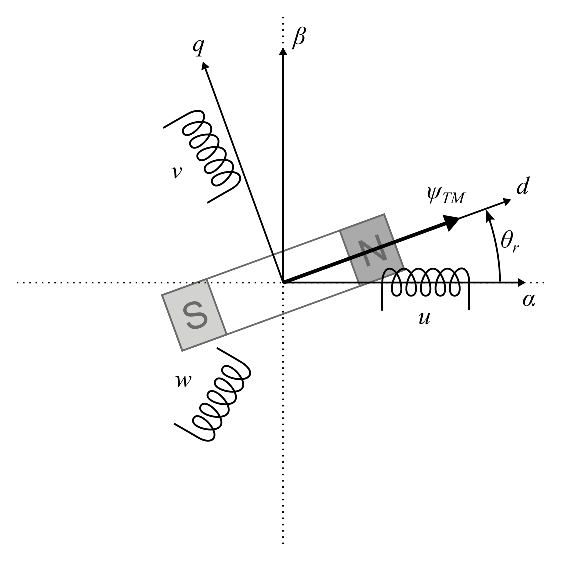
\includegraphics[width=0.5\columnwidth]{Slike/Inkscape/IPMSMsimple.eps}
    \caption{\label{IPMSM} Presek IPMSM stroja.}
\end{figure}


\section{Model IPMSM} \label{motor}

V pogonu se uporablja simetričen trofazni stroj, katerega matematično opišemo v RKS s sledečima enačbama:

\begin{equation} \label{motorModelD}
    u_d = R_si_d+L_d\frac{di_d}{dt}-\underbrace{\omega L_qi_q}_{e_d}
\end{equation}

\begin{equation} \label{motorModelQ}
    u_q = R_si_q+L_q\frac{di_q}{dt}+\underbrace{\omega L_di_d + \omega\Psi_{TM}}_{e_q}
\end{equation}

, kjer sta $e_d$ in $e_q$ inducirani napetosti vzdolžne in prečne komponente.
\\
Navor, ki ga tvori IPMSM pa je naslednji:

\begin{equation}
    M_{el} = \frac{3}{2}p\Bigl(\underbrace{\Psi_{TM}i_q}_{M_{sinhr}}+\underbrace{(L_d-L_q)i_qi_d}_{M_{rel}}\Bigr)
\end{equation}



\section{Brezsenzorsko vodenje FOC}

Za poenostavitev vodenja se uporablja Clarkina transformacija s katero trofazne veličine predstavimo v dveh ortogonalnih oseh - $\alpha$ in $\beta$ statorskega koordinatnega sistema (SKS). Veličine v
SKS pa transformiramo v RKS z uporabo Parkove transformacije, te pa se uporabljajo za vodenje tokov v vzdolžni in prečni osi. Pri Parkovi transformaciji poleg tokov potrebujemo tudi odklon RKS od SKS.
Ta se v senzorskih pogonih meri z dajalnikom pozicije, pri brezsenzorskih pa oceni iz merjenih veličin (tok in napetost). Na sliki \ref{koordinatniSistemSimple} so prikazani koordinatni sistemi, ki se
uporabljajo pri FOC vodenju. SKS je poravnan s statorjem, RKS z rotorjem in je od SKS odklonjen za kot $\theta_r$. FOC koordinatni sistem (FKS) pa je od SKS odklonjen za $\theta_f$ in se uporablja za
vodenje tokov. Napaka med dejanskim in ocenjenim ali pomerjenim odklonom rotorjem je $\Delta\theta$. 
\\
Pomerjeni tokovi stroja se v prvem koraku transformirajo v SKS z uporabo Clarkine transformacije, nato pa s Parkovo v FKS s kotom $\theta_f$. Tokove v FKS reguliramo, željeno prečno in vzdolžno
napetost regulatorja pa transformiramo v trifazne napetosti z inverzno Clarkino in Parkovo transformacijo. Željeni tok pa se uporablja za vodenje hitrosti, kjer je hitrost prav tako merjena ali
ocenjena.

\begin{figure}[!htbp]
    \centering
    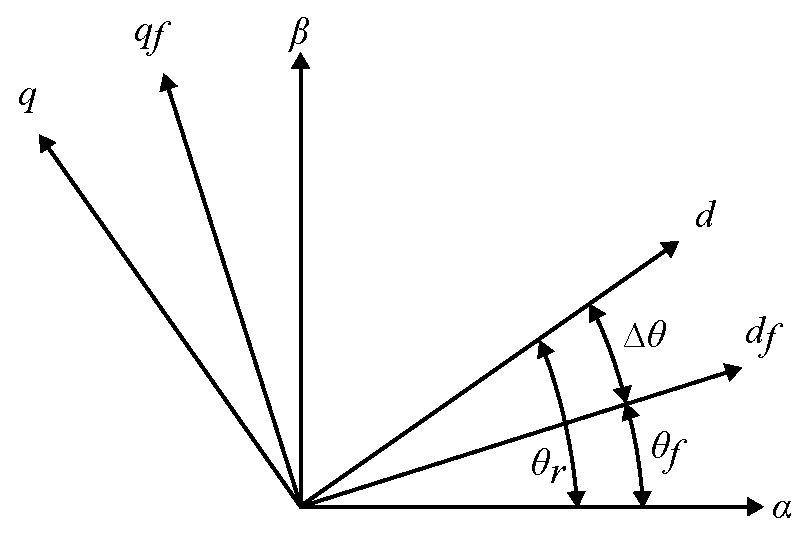
\includegraphics[width=0.7\columnwidth]{Slike/Inkscape/koordinatniSistemSimple.eps}
    \caption{\label{koordinatniSistemSimple} Uporabljeni koordinatni sistemi}
\end{figure}

Shema na sliki \ref{FOCshema} prikazuje brezsenzorsko vodenje, kjer se odklon in hitrost ocenjujeta, v primeru senzorskega pogona pa bi se merila.

\begin{figure}[!htbp]
    \centering
    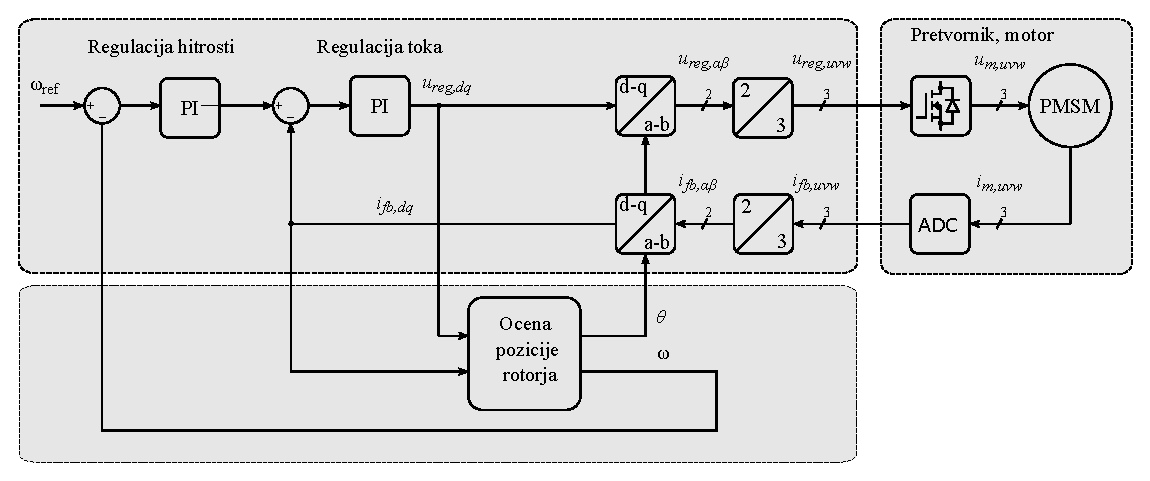
\includegraphics[width=1\columnwidth]{Slike/Inkscape/FOCsimple.eps}
    \caption{\label{FOCshema} Shema brezsenzorskega FOC vodenja.}
\end{figure}

Brezsenzorski algoritmi potrebujejo tudi začetno pozicijo rotorja, iz katere nadaljujejo ocenjevanje. Senzorski pogoni pozicijo merijo ves čas zato to, ni potrebno, v primeru brezsenzorskih pa napačna
začetna pozicija lahko pomeni, da se bo stroj vrtel v napačno smer. Ocenjevanje začetne pozicije je opisano v \cite{IPDBoussak}.

%Ker se uporablja brezsenzorsko vodenje, je potrebno odklon rotorja oceniti iz merjenega toka. Pri višji vrtilni hitrosti se za to uporablja opazovalnik pozicije. Ta z uporabo modela motorja,
%merjenega kota in znane pritisnjene napetosti oceni inducirano napetost, ki pa je funkcija odklona rotorja. Z uporabo fazno zaklenjene zanke (PLL) pa se iz inducirane napetosti oceni odklon
%rotorja.


%Opisana metoda odpove pri nižjih hotrostih, kjer je inducirana napetost premajhna oziroma ničelna v nevrtečem stanju. V takih pogojih se uporabljajo metode, ki izkoriščajo izraženost polov
%\cite{ThreeYearsOfExperience}. Skupnost vseh takih metod je vzbujanje statorja z dodatno napetostno komponento, ki je superponirana osnovno, ki tvori navor. Nekatere metode uporabljajo pulzirajoč
%signal, ki vzbuja le vzdolžno komponentno in tako minimizira moteč navor zaradi vzbujalne napetosti \cite{955987}. HFSI algoritem pa uporablja vrteč signal, ki vzbuja tudi prečno komponentno.
%
%Zaznavanje začetne pozicije rotorja v nevrtečem stanju je prav tako pomembna, saj omogoča takojšnje delovanje z visoko učinkovitostjo, prav tako pa izniči možnost vrtenja v napačno smer. Za zaznavanje
%začetne pozicije se prav tako izkorišča izraženost polov in je opisano v \cite{IPDBoussak}.


%================================================================================
%================================================================================
%**                             Delovanje HFSI                           
%================================================================================
%================================================================================
\chapter{Delovanje HFSI} \label{teorija}


%Na sliki \ref{hfsiMetoda} je prikazana shema HFSI algoritma.
%\begin{figure}[!htbp]
%    \centering
%    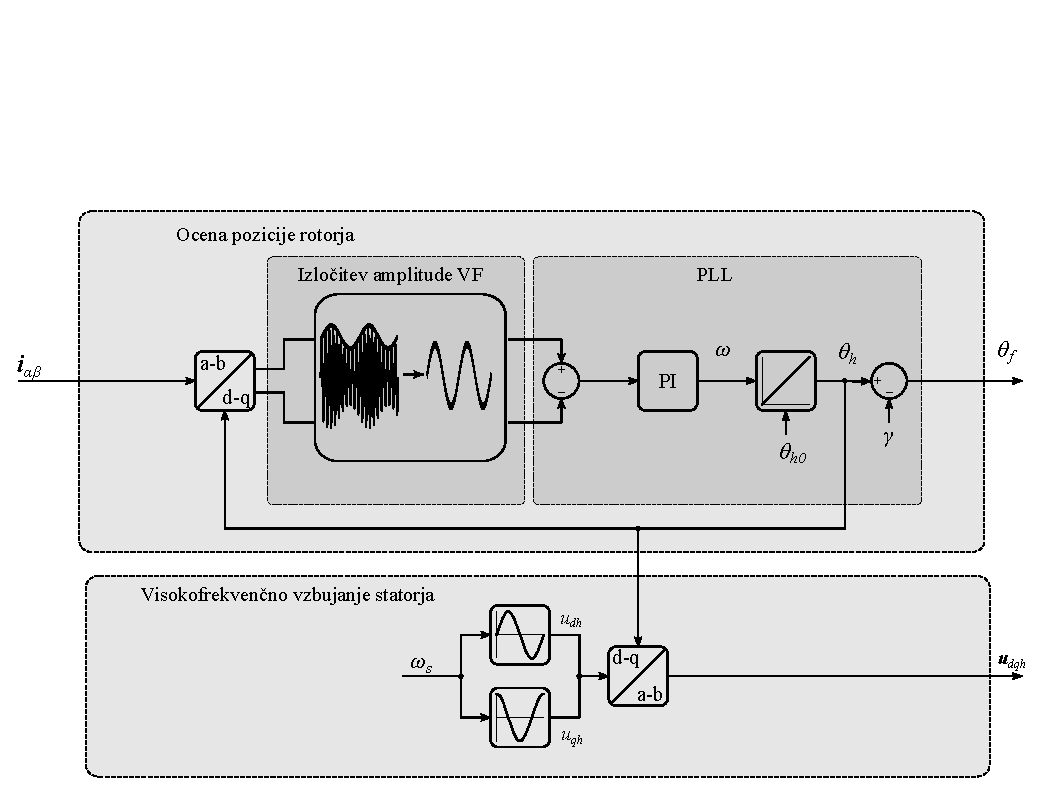
\includegraphics[width=0.9\columnwidth]{Slike/Inkscape/HFSIsimple.eps}
%    \caption{\label{hfsiMetoda} Shema HFSI algoritma.}
%\end{figure}
V klasičnem FOC vodenju trofaznega stroja se trofazne veličine z uporabo Clarkine transformacije pretvorijo v SKS, nato pa z uporabo Parkove transformacije v FKS. Pri HFSI metodi pa se uporablja
dodaten d-q koordinatni sistem, HFSI koordinatni sistem (HKS), v katerem vzbujamo stator z visokofrekvenčnim signalom in tokovni odziv uporabljamo za oceno odklona HKS. Na sliki
\ref{koordinatniSistem} je prikazan RKS, FKS s koordinatama $d_f$ in $q_f$ in HFSI koordinatni sistem s koordinatama $d_h$ in $q_h$, ki je od FKS zamaknjen za kot $\gamma$. Na sliki ima RKS prikazano
induktivnostno ovojnico, preko katere ocenjujemo pozicijo rotorja.

\begin{figure}[!htbp]
    \centering
    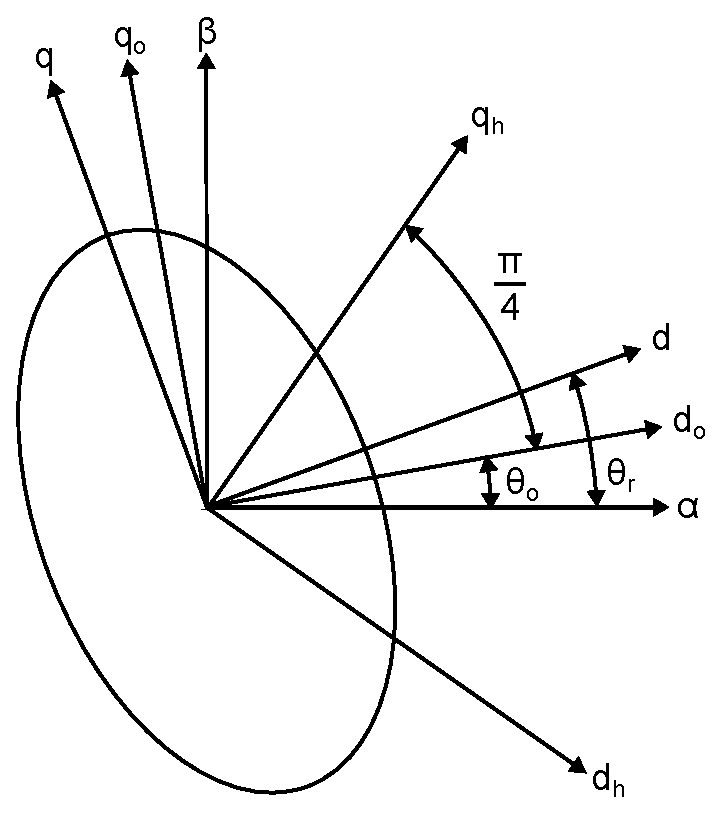
\includegraphics[width=0.7\columnwidth]{Slike/Inkscape/koordinatniSistem.eps}
    \caption{\label{koordinatniSistem} HFSI koordinatni sistem in induktivnostna ovojnica}
\end{figure}

%*******************************************************************************
%**                       Induktivnost stroja                               
%*******************************************************************************
\section{Induktivnost stroja}
Razlika induktivnosti v vzdolžni in prečni smeri RKS se pojavi zaradi neheterogene sestave rotorja in je maksimalna v prečni smeri in minimalna v smeri vzdolžni. Kot je prikazano na sliki
\ref{koordinatniSistem}, je HKS zamaknjen za kot $\gamma$ od FKS. Induktivnosti lahko matematično zapišemo kot:

\begin{equation}
    L_{dh} = L_p + L_r cos(2\Delta\theta + \gamma)
\end{equation}
\begin{equation}
    L_{qh} = L_p - L_r cos(2\Delta\theta + \gamma)
\end{equation}

, kjer je $\Delta\theta$ napaka ocene pozicije.
\\
Zapis induktivnosti s kosinusoidno funkcijo je le poenostavitev realnosti, ker niso vsi stroji konstruirani tako, da potek sledi sinusoidni krivulji. Oblika induktivnosti je namreč posledica
geometrije rotorja - oblike izraženih polov rotorja. Dejanski potek induktivnosti je prikazan na sliki \ref{induktivnostStroja}, kjer je bila ta pomerjena z RLC metrom ene same faze, drugi dve pa sta
bili odklopljeni. 

\begin{figure}[!htbp]
    \centering
    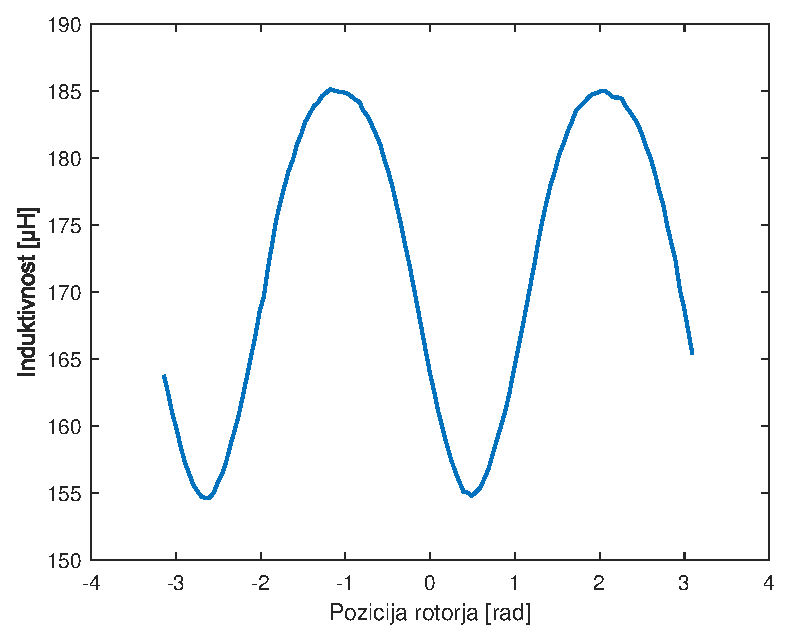
\includegraphics[width=0.80\columnwidth]{Slike/induktivnostStroja.eps}
    \caption{\label{induktivnostStroja} Induktivnost stroja. }
\end{figure}

%*******************************************************************************
%**                     Visokofrekvenčno vzbujanje statorja                             
%*******************************************************************************
\section{Visokofrekvenčno vzbujanje statorja}

% TODO dodaj dejansko vzbujanje

Ker je induktivnost stroja odvisna od pozicije rotorja, lahko za ocenjevanje pozicije to uporabimo. Stator vzbujamo z visokofrekvenčnim signalom, amplituda tokovnega odziva pa bo odvisna od
induktivnosti. 

V enačbah \ref{motorModelD} in \ref{motorModelQ} ob predpostavitvi, da se rotor ne vrti oziroma vrti z nizko frekvenco, zanemarimo člena $e_d$ in $e_q$ in stroj poenostavimo v RL vezje:

\begin{equation}
    u_d = R_si_d+L_d\frac{di_d}{dt}
\end{equation}

\begin{equation}
    u_q = R_si_q+L_q\frac{di_q}{dt}
\end{equation}

% profesor: Na sestanku sva rekla da bi tukaj izhajal iz enačb motorja, saj sistem opazujemo pri frekvenci vzbujalnega signala in ker člena "inducirane" napetosti vsebujeta vrtilno hitrost (sta z njo
% množena) ju lahko enačim z nič. Vendar pa nisem več prepričan v to, saj imata iq in id še vedno visokofrekvenčno komponento. Ko se bo motor vrtel bom tako s prečnim tokom "motil" vzdolžnega in
% obratno, kjer bo to vedno hujše z višjimi obrati. 

Pri dovolj visoki frekvenci vzbujanja se tudi predpostavi, da je statorska ohmska upornost mnogokrat manjša od reaktance in zapišemo amplitudo tokovnega odziva vzdolžne in prečne komponente HKS
odvisne od induktivnosti.

\begin{equation}
    I_{dh} = \frac{U_h}{\omega_sL_{dh}}
\end{equation}

\begin{equation}
    I_{qh} = \frac{U_h}{\omega_sL_{qh}}
\end{equation}

Ko vstavimo induktivnosti $L_{dh}$ in $L_{qh}$ v zgornjo enačbo, dobimo amplitudo tokovnega odziva v odvisnosti od odklona HKS od RKS.
\begin{equation} \label{tokovniOdzivEnacbaD}
    I_{dh} = \frac{U_d}{\omega_s (L_p + L_r cos(2\Delta\theta + \gamma))}
\end{equation}

\begin{equation}\label{tokovniOdzivEnacbaQ}
    I_{qh} = \frac{u_s}{\omega_s (L_p - L_r cos(2\Delta\theta + \gamma))}
\end{equation}

Amplitudo na realnem sistemu izračunamo s Furierovo transformacijo merjenega toka, kjer se v digitalnih sistemih velikokrat uporablja diskretna Fourierova transformacija (DFT). Ta pa je za ta primer
prepotratna, saj potrebujemo amplitudo signala pri le eni frekvenci - zato uporabimo fourierovo vrsto. Do amplitude pridemo z množenjem okna s sinusno in kosinusno funkcijo
\cite{enwiki:fourierSeries}. 

Na sliki \ref{tokovniOdzivKot0} sta amplitudi VF tokovnega odziva v prečni in vzdolžni osi, kjer je bil odklon HKS od FKS, kot $\gamma$, enak nič. Ko je odklon FKS od RKS ali napaka ocene rotorja
$\Delta\theta$ enaka nič, bo amplituda v vzdolžni smeri maksimalna, v prečni pa minimalna. Če želimo tekom delovanja stroja ohranjati minimalno napako ocene pozicije rotorja, moramo tako poskrbeti, da
bosta imeli amplitudi maksimalno in minimalno vrednost. Ta rešitev pa ni optimalna, saj ob neki napaki ocene in tako s prehodom izven maksimalne amplitude v nižjo vrednost težko vemo, ali je napaka
pozitivna ali negativna. Drugače rečeno, če si predstavljamo graf na sliki \ref{tokovniOdzivKot0} kot odvisnost amplitud od napake ocene rotorja, iz merjenih amplitud ne moremo razlikovati med
pozitivno in negativno napako. To pa pomeni, da ne vemo v katero smer moramo popraviti kot, da pridemo nazaj na maksimalno vrednost.

\begin{figure}[!htbp]
    \centering
    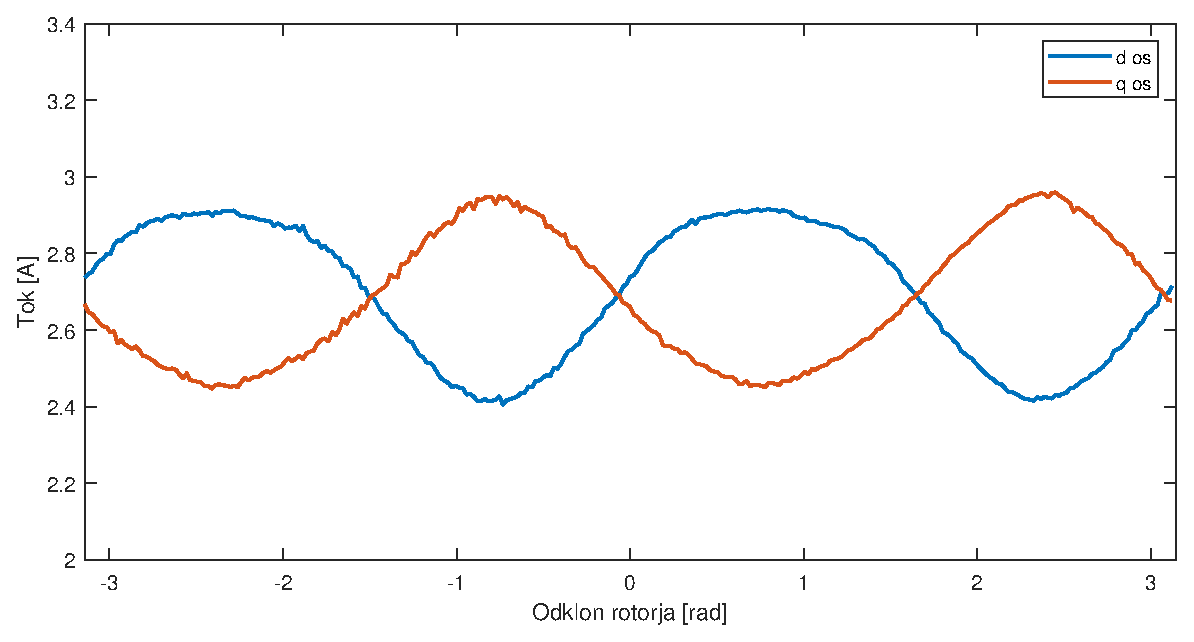
\includegraphics[width=0.95\columnwidth]{Slike/tokovniOdzivKot0.eps}
    \caption{\label{tokovniOdzivKot0} $I_{dh}$ in $I_{qh}$ pri $\gamma = 0$.}
\end{figure}

Ko pa postavimo kot $\gamma$ na $\frac{pi}{4}$, torej je HKS za ta kot odmakjnen od FKS, pa bosta amplitudi ob ničti napaki enaki. Če amplitudi odštejemo, bo brez napake ocene njuna razlika enaka nič,
pri pozitivni napaki bo razlika pozitivna, pri negativni napaki pa negativna. Zato postavimo $\gamma$ na vrednost $\frac{pi}{4}$, njena vrednost pa skozi delovanje algoritma ne bo sprinjala in bo
konstantna.

\begin{figure}[!htbp]
    \centering
    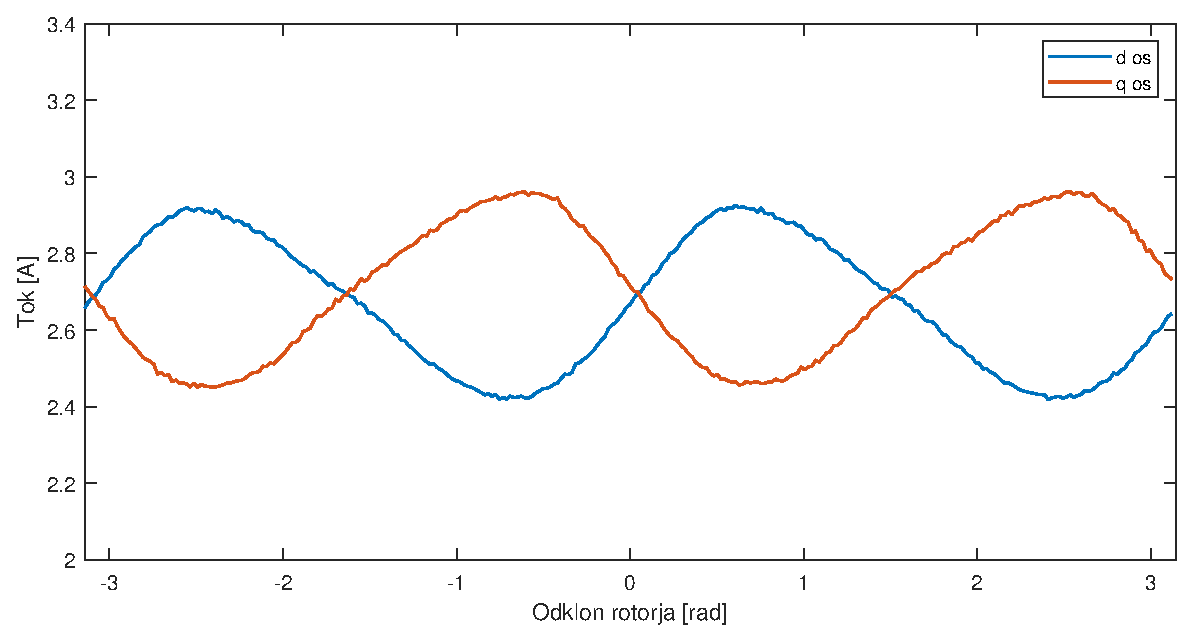
\includegraphics[width=0.95\columnwidth]{Slike/tokovniOdzivKot45.eps}
    \caption{\label{tokovniOdzivKot45} $I_{dh}$ in $I_{qh}$ pri  $\gamma = \frac{pi}{4}$.}
\end{figure}

%*******************************************************************************
%**                      Izračun pozicije rotorja                               
%*******************************************************************************
\section{Izračun pozicije rotorja}

Amplitudi VF tokovnega odziva na prečni in vzdolžni osi HKS sedaj odštejemo in to razliko uporabimo kot regulirano veličino:

\begin{equation}
    I_e = I_{dh} - I_{qh}
\end{equation}

\begin{figure}[!htbp]
    \centering
    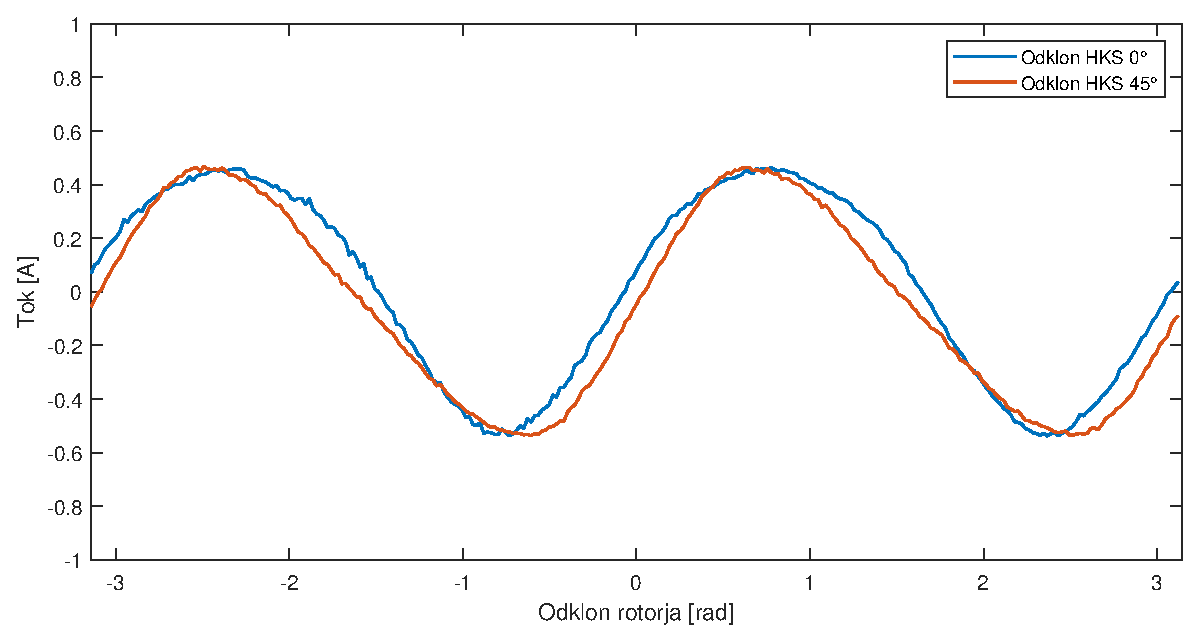
\includegraphics[width=1\columnwidth]{Slike/reguliranaVelicinaIdq0.eps}
    \caption{\label{reguliranaVelicinaIdq0} $I_e$ pri odklonu 0° in 45°.}
\end{figure}

Na sliki \ref{reguliranaVelicinaIdq0} je prikazan tok $I_e$, kjer je $\gamma$ enaka $\frac{\pi}{4}$. Ker je ta veličina odvisna od relativne pozicije rotorja od HKS, lahko to veličino reguliramo in s
tem ocenjujemo odklon rotorja. Ko je ocena brez napake, je razlika amplitud oziroma regulirana veličina enaka nič, zato bo tudi željena vrednost regulacije nič. 

Od željene vrednosti regulirane veličine odštejemo dejansko vrednost $I_e$ in to vstavimo v PI regulator. Izhod regulatorja je regulirna veličina, to je veličina s katero vplivamo na regulirano. 
V tem primeru je to vrtilna hitrost $\omega_h$, ki jo integriramo da dobimo pozicijo HKS, katero pa v povratni zanki uporabimo za nov izračun $I_e$. 

Tako z regulacijo $I_e$ na nič dosežemo, da sta amplitudi tokovnega odziva v vzdolžni in prečni komponenti HKS enaki, s tem pa dejanska pozicija rotorja enaka ocenjeni poziciji. 
Ker pa to velja za primer, ko ima $\gamma$ vrednost $\frac{\pi}{4}$, pridemo do ocene pozicije rotorja z izračunom:

\begin{equation}
    \theta_{f} = \theta_{h} - \frac{\pi}{4}
\end{equation}

Točke, kjer ima $I_e$ vrednost 0, lahko imenujemo stabilne točke, saj se z odklonom izven tega območja zaradi regulatorja premaknemo nazaj v stabilnost.






%*******************************************************************************
%**                      Odstopanja realnega sistema                           
%*******************************************************************************
\section{Odstopanja realnega sistema}
%Kot induktivnost stroja, so tudi tokovni odzivi poenostavitev realnega sistema. Lahko pričakujemo najnižjo vrednost amplitude tokovnega odziva v vzdolžni smeri in najvišjo v prečni, vendar bo oblika
%in s tem tudi odklon, kjer sta odziva enake amplitude malo zamaknjena od pričakovane. To je prikazano na slikah \ref{tokovniOdzivKot0} in \ref{tokovniOdzivKot45}, kjer je odklon rotorja kot med
%rotorjem - gnanim ročno - in FKS (HKS je za pi/4 zamaknjen od FKS).

Tekom razvoja smo opazili, da amplitude v določenih razmerah začnejo odstopati od pričakovanih. Že na slikah \ref{tokovniOdzivKot0} in \ref{tokovniOdzivKot45} lahko opazimo, da obliki potekov amplitud
nista enaki. Na prvi sliki je bil HKS poravnan s SKS, na drugi pa je bil za $\frac{\pi}{4}$ odmaknjen. V idealnem okolju, bi pričakovali enaki obliki, le zamaknjeni za $\frac{\pi}{4}$, vendar pa se
oblika signala spreminja z odklonom HKS od SKS. Slika \ref{reguliranaVelicinaIdq0in45} prikazuje $I_e$ pri teh dveh meritvah, kjer sta bili meritvi poravnani. Opazimo, da se s spremembo oblike
premakne stabilna točka.

\begin{figure}[!htbp]
    \centering
    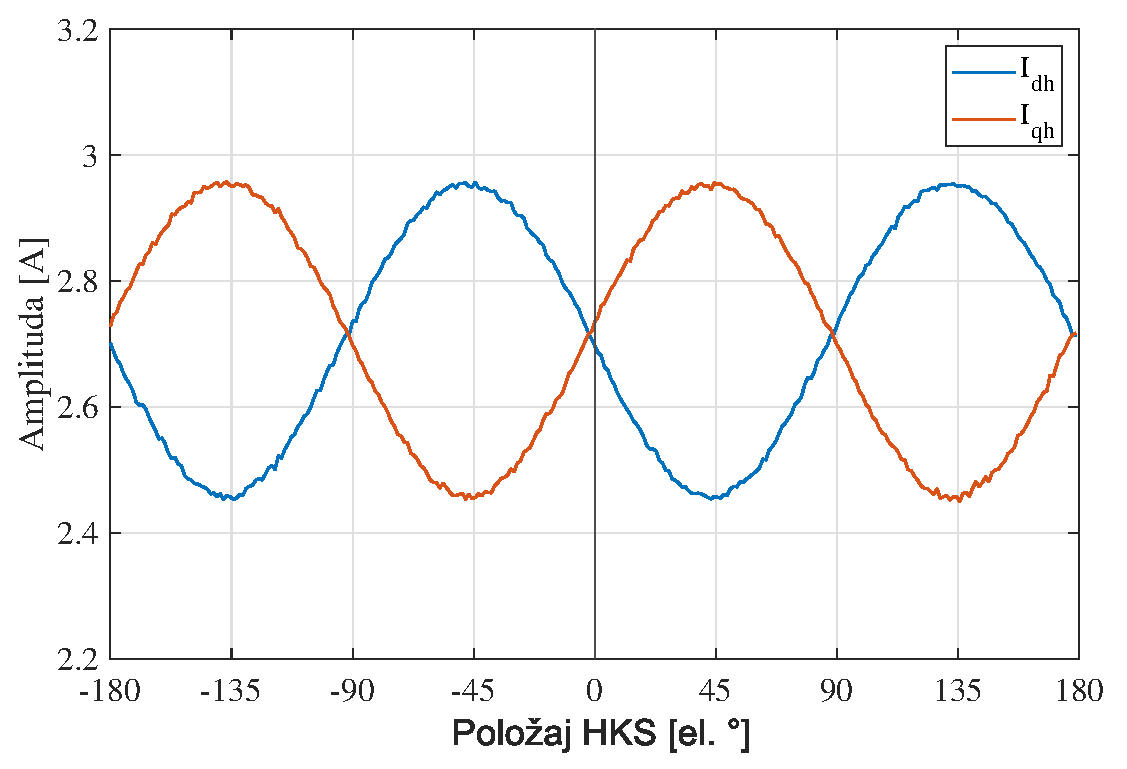
\includegraphics[width=1\columnwidth]{Slike/reguliranaVelicinaIdq0in45.eps}
    \caption{\label{reguliranaVelicinaIdq0in45} $I_e$ pri odklonu HKS 0° in 45°.}
\end{figure}

Na sliki \ref{reguliranaVelicinaIdq0in45} je bila enosmerna komponenta prečnega in vzdolžnega toka nič, stator smo vzbujali le z VF signalom za ocenjevanje pozicije. Za tvorjenje navora pa potrebujemo
neničelno enosmerno prečno komponentno, katere vpliv na tok $I_e$ je prikazan na sliki \ref{reguliranaVelicinaIs}. Prečna komponenta je bila vodena s FOC regulatorji toka v koordinatnem sistemu FKS.
Vzdolžna komponenta je bila v FKS enaka nič, v RKS pa ne, saj smo z odklanjanjem rotorja RKS odmaknili od FKS in se prečna komponenta v FKS preslika v prečno in vzdolžno komponento RKS. Na sliki se
vidi, da z višanjem prečne komponente postane v določenih smereh $I_e$ bolj izrazit v drugih pa bolj položen. Bolj pomembno pa je spreminjanje oblike in naklon $I_e$ okoli stabilne točke, kjer bo delovna točka našega
sistema. Z nekim odstopom okoli ničelne napake se bo $I_e$ premikal po krivilji in sprememba naklona pomeni spremembo ojačanja povratne zanke, to pa pomeni spremembo dinamike sistema. Naklon se s
prečnim tokom sicer ne spreminja, lahko pa opazimo, da se z negativnim prečnim tokom (vrtenje v nasprotno smer) $I_e$ okoli delovne točke ne spreminja linearno. To nam lahko okvari delovanje in terja
postavitev delovne točke v drugo stabilno lego.

% profesor: zadnji stavek spustim? Če pustim izjavo "postavitev delovne točke v drugo stabilno lego" rabim to potrditi in pokazati delovanje v primeru ko ne prestavim delovne točke?

\begin{figure}[!htbp]
    \centering
    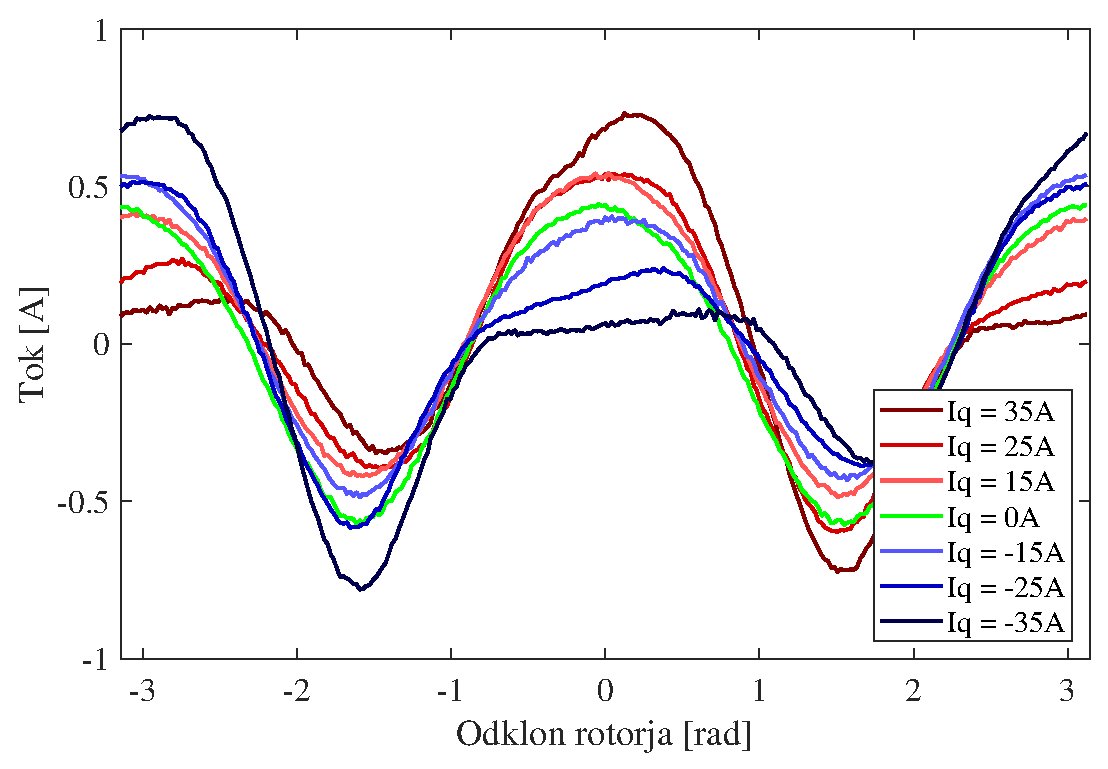
\includegraphics[width=1\columnwidth]{Slike/reguliranaVelicinaIs.eps}
    \caption{\label{reguliranaVelicinaIs} Vpliv enosmerne prečne tokovne komponentne na $\hat{i}_{e}$ pri različnih odklonih rotorja od FKS.}
\end{figure}




Ta pojav lahko bolj podrobno pogledamo z meritvijo $I_e$, ko je FKS poravnan z RKS, ki je merjen z dajalnikom pozicije. Pričakovali bi, da bi bila $I_e$
na vseh pozicijah rotorja enaka nič, saj je v tem primeru nimamo napake ocene. Realna meritev pa pokaže na pojav višjeharmonskega popačenja, kot je prikazano na sliki
\ref{tokovniOdzivIs_HKSslediRKS_diff}, kjer je bilo opravljenih več meritev pri različnih prečnih tokovih. Opazimo, da višjeharmonsko popačenje narašča z večanjem prečnega toka.

\begin{figure}[!htbp]
    \centering
    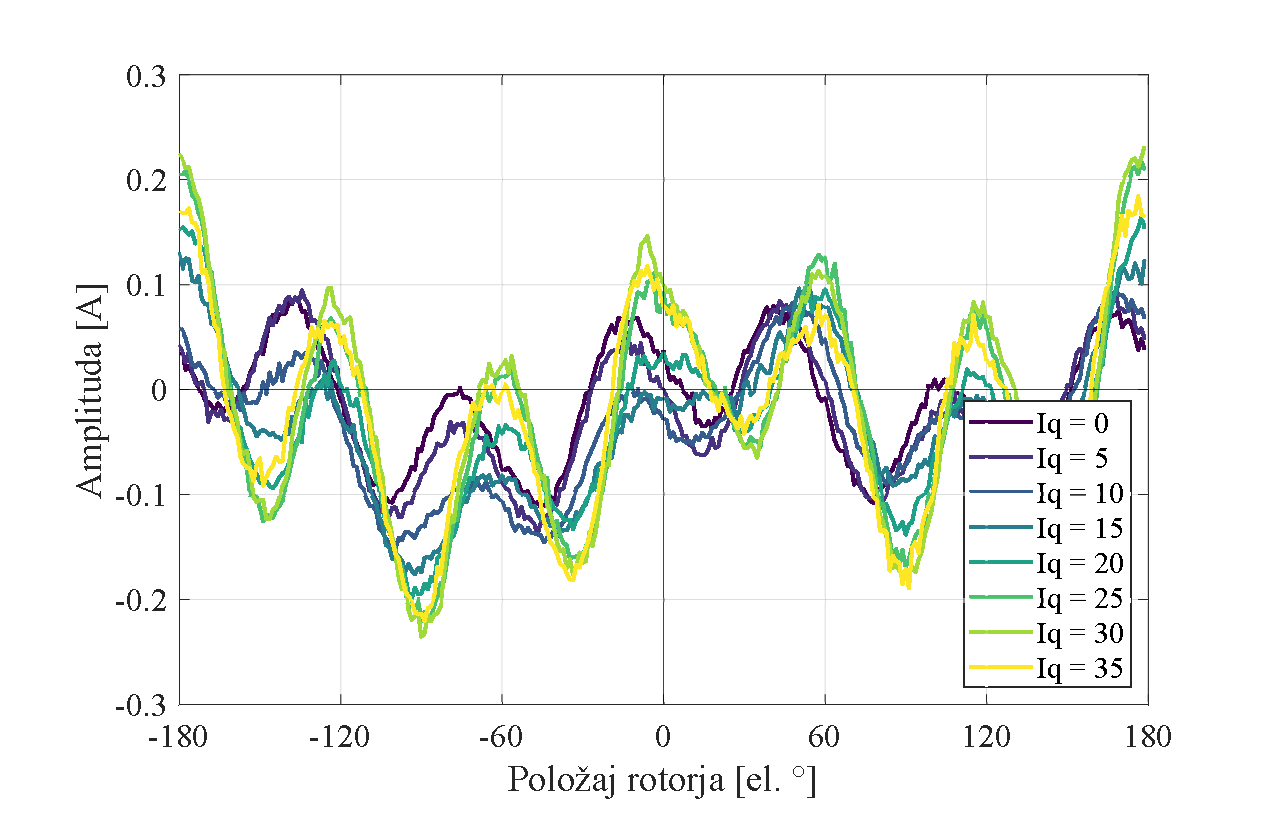
\includegraphics[width=1\columnwidth]{Slike/tokovniOdzivIs_HKSslediRKS_diff.eps}
    \caption{\label{tokovniOdzivIs_HKSslediRKS_diff} Neidealnost $\hat{i}_{e}$ pri različnih prečnih tokovih, kjer HKS sledi RKS.}
\end{figure}

V prejšnjem poglavju je so bile meritve zajete v primeru, kjer imata vzdolžna in prečna komponenta le VF vzbujalni signal za ocenjevanje pozicije rotorja. Slika 



Moramo pa se zavedati tudi dejstva, da pri brezsenzorskem vodenju ne poznamo prave pozicije rotora in imamo na voljo samo približno vrednost. Slike \ref{tokovniOdzivId} - \ref{tokovniOdzivIq_IqAmp},
kjer je bila pozicija rotorja znana z dajalnikom pozicije, prikazujejo samo odziv amplitude VF tokovnega odziva v primeru vzdolžnega ali prečnega toka RKS. V realnem sistemu pa se bo pozicija
ocenjevala in bo imela neko napako. Tudi v poenostavljenem vodenju kjer uporabljamo samo prečni tok za tvorjenje navora, bomo v primeru napake ocenjene pozicije rotorja v RKS imeli nek neničelni
vzdolžni tok, saj prečni tok, ki ga vodimo s FOC vodenjem, vodimo v FKS in ne v RKS, s prisotno napako ocenjenega toka pa ta dva nista poravnana. Zato si poglejmo amplitude tokovnih odzivov v primeru,
kjer ne poznamo pozicije rotorja. HKS je kot prej od FKS odmaknjen za $\frac{\pi}{4}$ in poravnan s SKS, vrednost prečnega toka je parametrizirana, vzdolžni tok se vodi na ničelno vrednost, z vrtenjem
rotorja pa umetno ustvarjamo napako ocene pozicije.

\begin{figure}[!htbp]
    \centering
    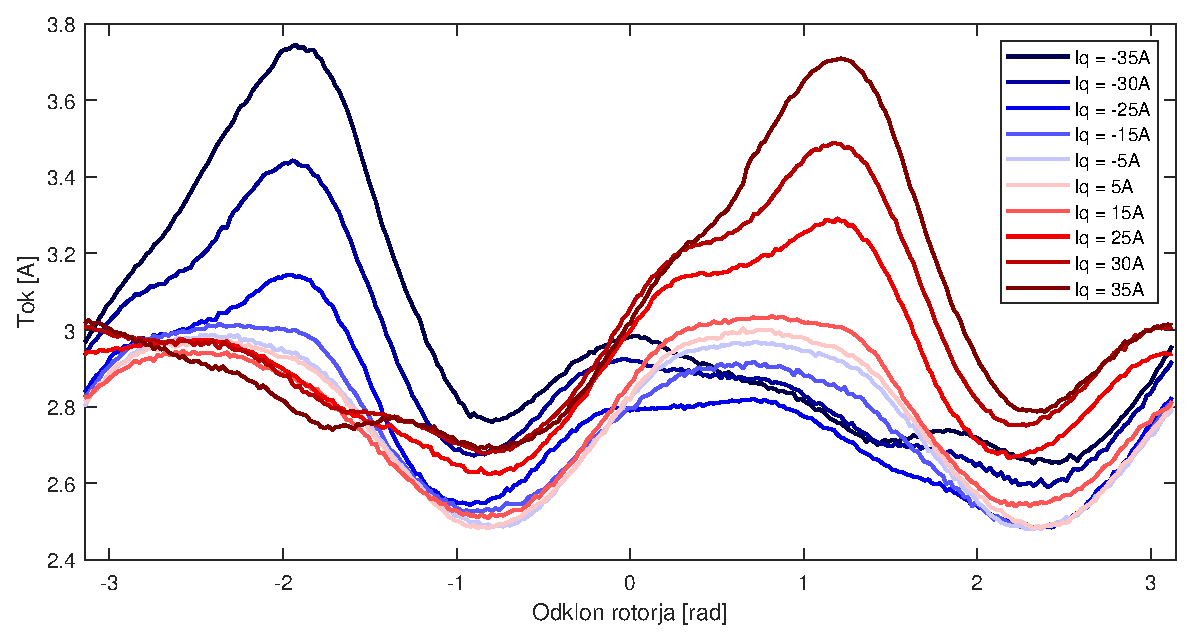
\includegraphics[width=0.95\columnwidth]{Slike/tokovniOdzivIs_IdAmp.eps}
    \caption{\label{tokovniOdzivIs_IdAmp} Vpliv enosmerne prečne tokovne komponentne na $\hat{i}_{dh}$ pri različnih odklonih rotorja od FKS.}
\end{figure}

\begin{figure}[!htbp]
    \centering
    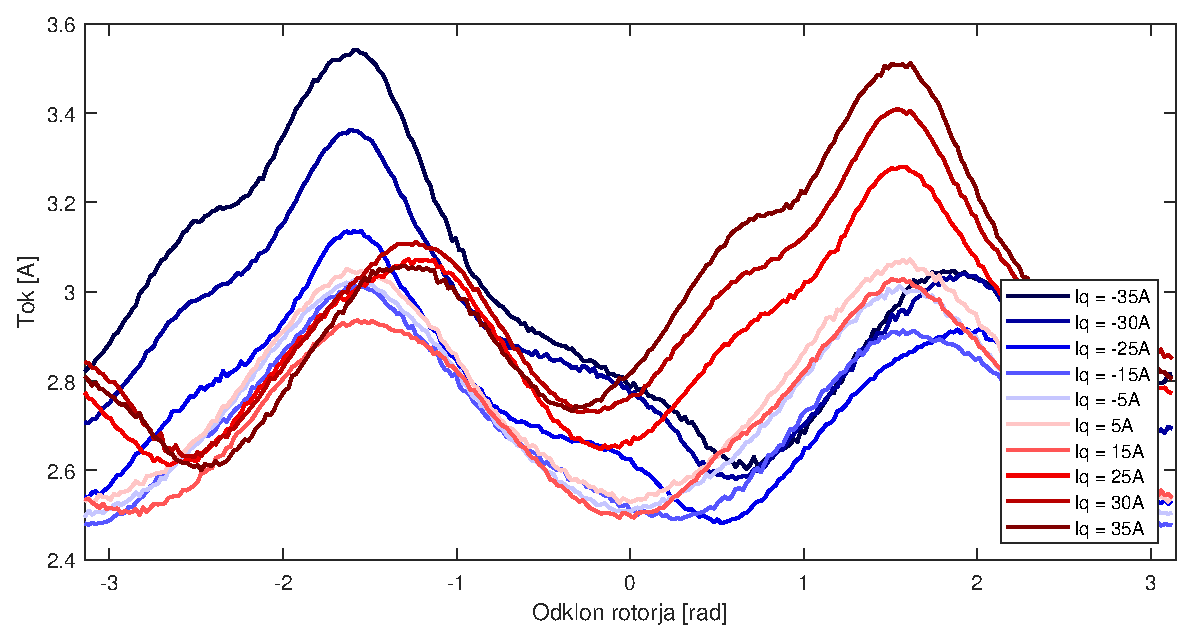
\includegraphics[width=0.95\columnwidth]{Slike/tokovniOdzivIs_IqAmp.eps}
    \caption{\label{tokovniOdzivIs_IqAmp} Vpliv enosmerne prečne tokovne komponentne na $\hat{i}_{qh}$ pri različnih odklonih rotorja od FKS.}
\end{figure}

Na sliki \ref{tokovniOdzivIs_IdAmp} je prikazana amplituda VF tokovnega odziva v vzdolžni smeri, na sliki \ref{tokovniOdzivIs_IqAmp} pa v prečni. Opazimo, da so odzivi pri negativnem toku le fazno
zamaknjeni za 180 stopinj. To je pričakovano, saj je negativni tok le za 180 električnih stopinj obrnjen vektor pozitivnega prečnega toka. Opazimo tudi, da je v eni polovici grafa amplituda dokaj
nespremenljiva, na drugem koncu pa močno odvisna od odklona rotorja. Enosmerna komponenta prečnega toka je regulirana v FKS, kateri pa se ne obrača relativno na SKS, kar pomeni, da z obračanjem
rotorja v nekaterih pozicijah tvorimo navor, v drugih pa rotor magnetimo s tem tokom. V primeru, kjer je napaka ocene majhna, je magnetenje rotorja tudi majhno saj je le prečni tok neničeln.

Dodatna meritev, ki pokaže ne-idealnost sistema je primer, kjer HKS odmaknemo od RKS za $\frac{\pi}{4}$ - torej morata biti amplitudi tokovnega odziva v HKS enaki (lahko rečemo tudi da FKS poravnamo z
RKS, katerega pozicija je znana z dajalnikom in obratujemo brez napake ocene pozicije rotorja). Prečni tok parametriziramo in opazujemo njegov vpliv na amplitudi. Odklon RKS od SKS je znan in merjen z
dajalnikom pozicije, nato pa rotor počasi vrtimo.  V idealnem primeru bi morali dobiti konstanten odziv enakih amplitud v obeh smereh, vendar zaradi raznih vplivov dobimo na odzivu motnje, ki kvarijo
oceno pozicije. To je prikazano na slikah \ref{tokovniOdzivIs_HKSslediRKS_IdAmp} - \ref{tokovniOdzivIs_HKSslediRKS_IqAmp}, kjer je prikazana amplituda v vzdolžni smeri
(\ref{tokovniOdzivIs_HKSslediRKS_IdAmp}) in prečni smeri (\ref{tokovniOdzivIs_HKSslediRKS_IqAmp}).
\newpage

\begin{figure}[!htbp]
    \centering
    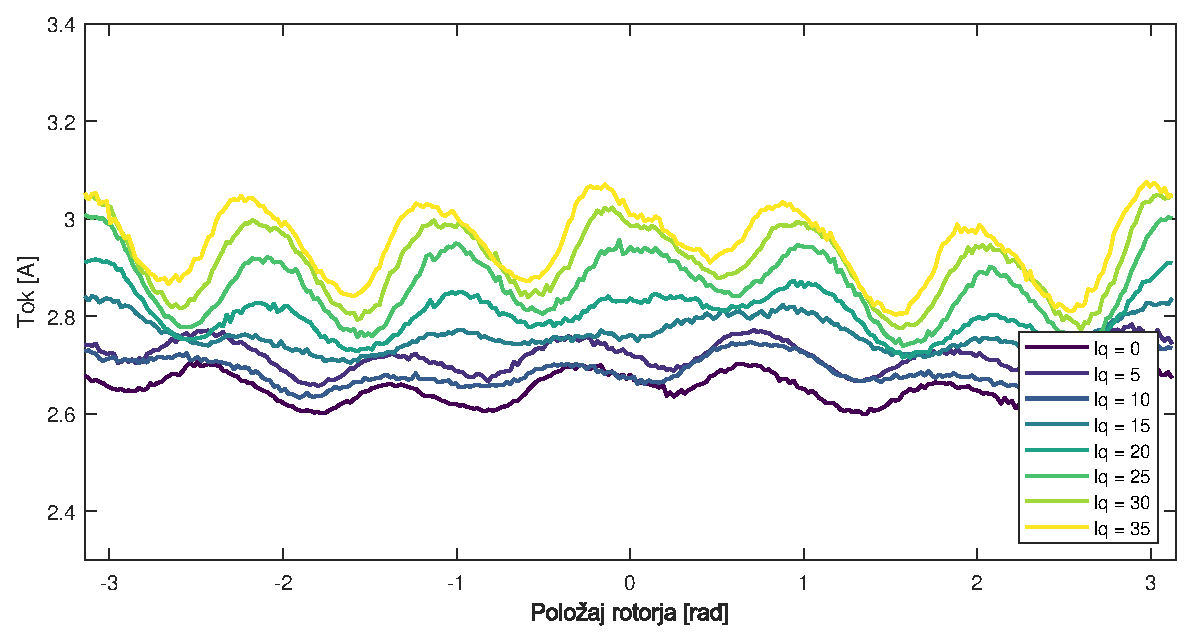
\includegraphics[width=0.95\columnwidth]{Slike/tokovniOdzivIs_HKSslediRKS_IdAmp.eps}
    \caption{\label{tokovniOdzivIs_HKSslediRKS_IdAmp} Neidealnost $\hat{i}_{dh}$ pri različnih prečnih tokovih, kjer HKS sledi RKS.}
\end{figure}

\begin{figure}[!htbp]
    \centering
    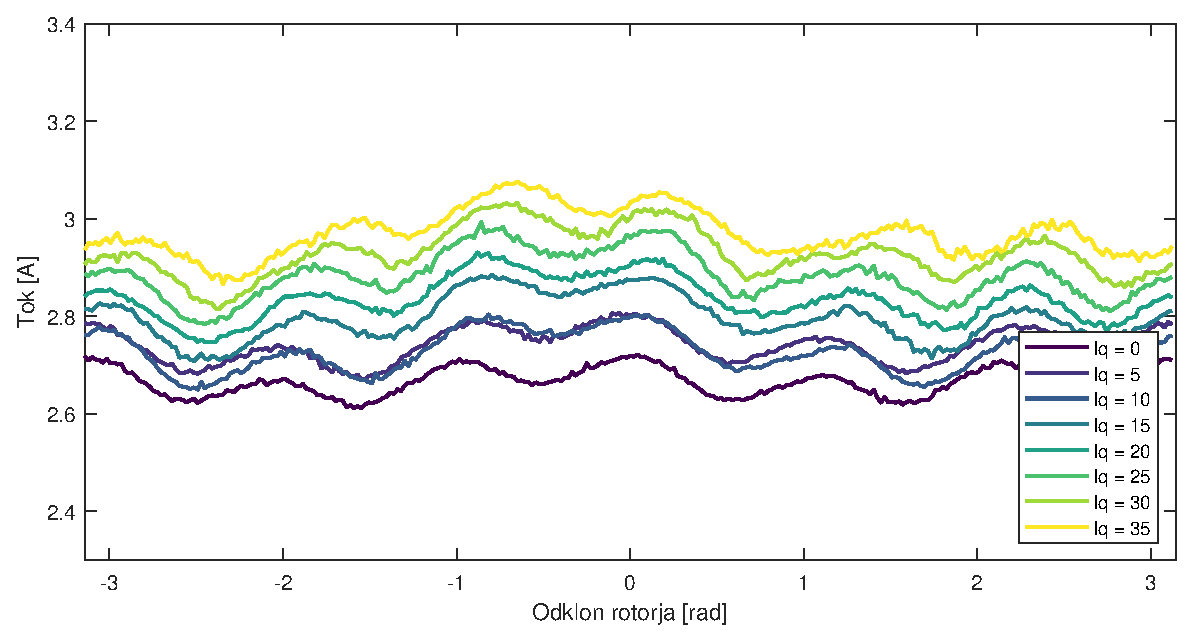
\includegraphics[width=0.95\columnwidth]{Slike/tokovniOdzivIs_HKSslediRKS_IqAmp.eps}
    \caption{\label{tokovniOdzivIs_HKSslediRKS_IqAmp} Neidealnost $\hat{i}_{qh}$ pri različnih prečnih tokovih, kjer HKS sledi RKS.}
\end{figure}

Najprej se opazi, da se povprečna amplituda z višanjem prečnega toka povečuje, bolj pomembno pa je izrazito povečanje višje-harmonske komponente, ki se pojavi v vzdolžnem odzivu. Ta pride do izraza v
naslednjem poglavju, kjer uvedemo novo spremenljivko - razliko amplitud tokovnih odzivov.

%*******************************************************************************
%**                      Vpliv mrtvega časa pretvornika                           
%*******************************************************************************
\section{Vpliv mrtvega časa pretvornika}

V praktičnem sistemu, kjer se uporablja močnostni pretvornik imamo opravka s preklopi visokih in nizkih tranzistorjev. Ko je odprt nizek fet, je fazna napetost 0V, ko je odprt visok fet pa je fazna
napetost enaka napajalni. Med preklopom iz 0V in 24V pa je za kratek čas potrebno izklopiti oba, saj v primeru, kjer prevajata oba nastane nizko-impedančna pot, ki povzroči kratek stik. Čas, ko sta
izklopljena oba se imenuje mrtvi čas, napetost faze v tem času pa je odvisna od smeri toka te faze. Slika \ref{mrtviCasRazlaga} prikazuje odvisnost napetosti faze, ko sta oba tranzistorja močnostnega
pretvornika te faze zaprta. Ker sta oba zaprta, mora tok steči skozi diodo zgornjega ali spodnjega tranzistorja. Ko tok teče v stroj, steče skozi spodnjo diodo, zato je napetost te faze v tem primeru
0V, ko pa teče iz stroja, pa steče skozi zgornjo in je napetost takrat enaka napajalni. To povzroča napetostno napako \cite{ambrovzivc2016elektrivcni}.

\begin{figure}[!htbp]
    \centering
    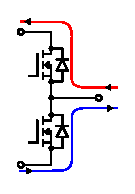
\includegraphics[width=0.4\columnwidth]{Slike/Inkscape/mrtviCasRazlaga.eps}
    \caption{\label{mrtviCasRazlaga} Napetost faze ko sta oba tranzistorja zaprta}
\end{figure}

Za delovanje HFSI algoritma pa poleg osnovne harmonske komponente za tvorjenje navora vzbujamo stator še z visoko frekvenčno komponento. V primeru, kjer stator vzbujamo samo z visoko frekvenco, bi
mrtvi čas vedno vplival na odziv in njegov vpliv bi bil konstanten. Ko pa vzbujamo še s konstantnim prečnim ali vzdolžnim tokom, pa vidimo vpliv mrtvega časa samo, ko osnovna harmonska tokovna
komponenta zamenja polariteto. To lahko potrdimo z meritvami na realnem sistemu, kjer HKS odmaknemo od RKS za $\frac{\pi}{4}$ in v FKS vzbujamo stator s konstantnim tokom, rotor pa počasi vrtimo.
Pričakovali bi konstantno in enako amplitudo VF tokovnega odziva v prečni in vzdolžni komponenti HKS, vendar na sliki \ref{mrtviCas} opazimo, da je na šestih pozicijah odziv popačen in da je magnituda
napake dokaj linearno odvisna od mrtvega časa. Modra barva označuje amplitudo VF odziva prečne komponente, rdeča pa vzdolžne. Temnejši kot so odzivi, večji je mrtvi čas. 

\begin{figure}[!htbp]
    \centering
    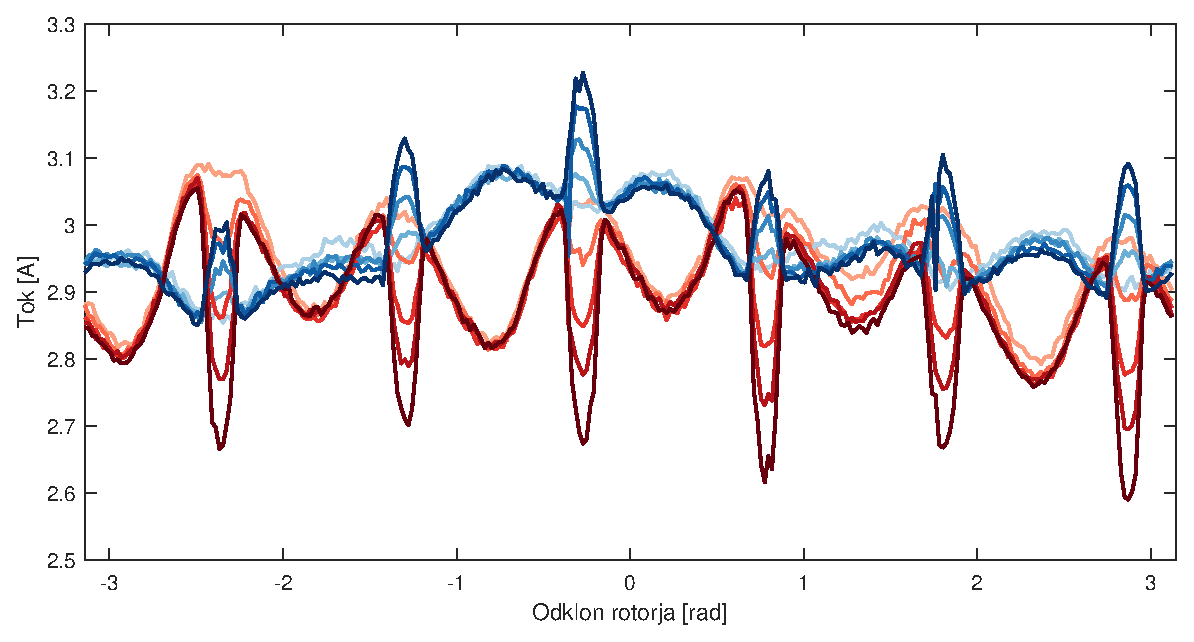
\includegraphics[width=0.95\columnwidth]{Slike/mrtviCas.eps}
    \caption{\label{mrtviCas} Odvisnost popačenja amplitude odziva od dolžine mrtvega časa}
\end{figure}

Prav tako lahko potrdimo, da je mrtvi čas odvisen od napajalne napetosti, prikazano na sliki \ref{mrtviCasNapetost}. Odziv je bil pomerjen pri napetostih 16V, 24V in 32V, kjer je temnejša barva večja
napetost.

\begin{figure}[!htbp]
    \centering
    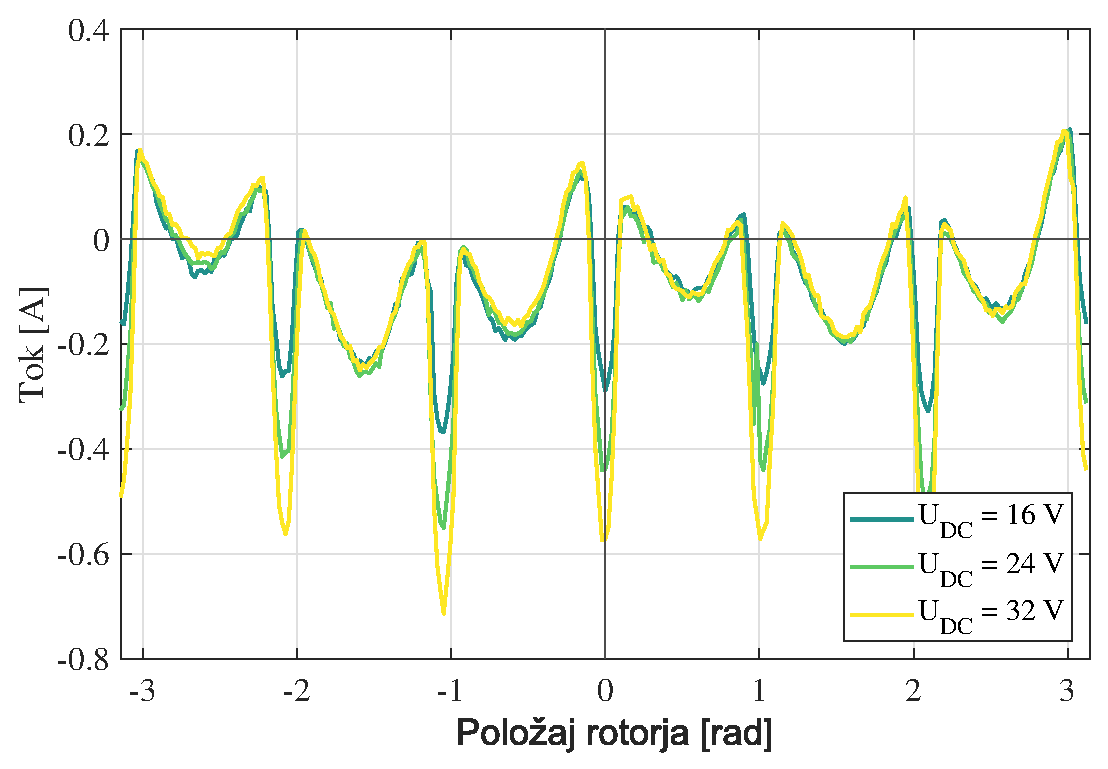
\includegraphics[width=0.95\columnwidth]{Slike/mrtviCasNapetost.eps}
    \caption{\label{mrtviCasNapetost} Odvisnost popačenja amplitude odziva od napajalne napetosti }
\end{figure}

Dodatno lahko pokažemo, da se vpliv mrtvega časa začne kazati takrat, ko začne VF tokovni odziv menjati polariteto. Na zgornjem grafu sta prikazani amplitudi tokovnega odziva prečne in vzdolžne
komponente in fazni tok $i_u$, na drugem grafu pa filtriran $i_u$ s pasovnim filtrom. Na prvem grafu je z modro barvo označen del, kjer fazni tok prehaja skozi nič, torej takrat, ko mrtvi čas kvari
tokovni odziv. Opazi se izrazit efekt mrtvega časa na tokovnem odzivu prečne in vzdolžne komponente v modrem delu, prav tako pa se opazi na faznem toku na drugem grafu.

\begin{figure}[!htbp]
    \centering
    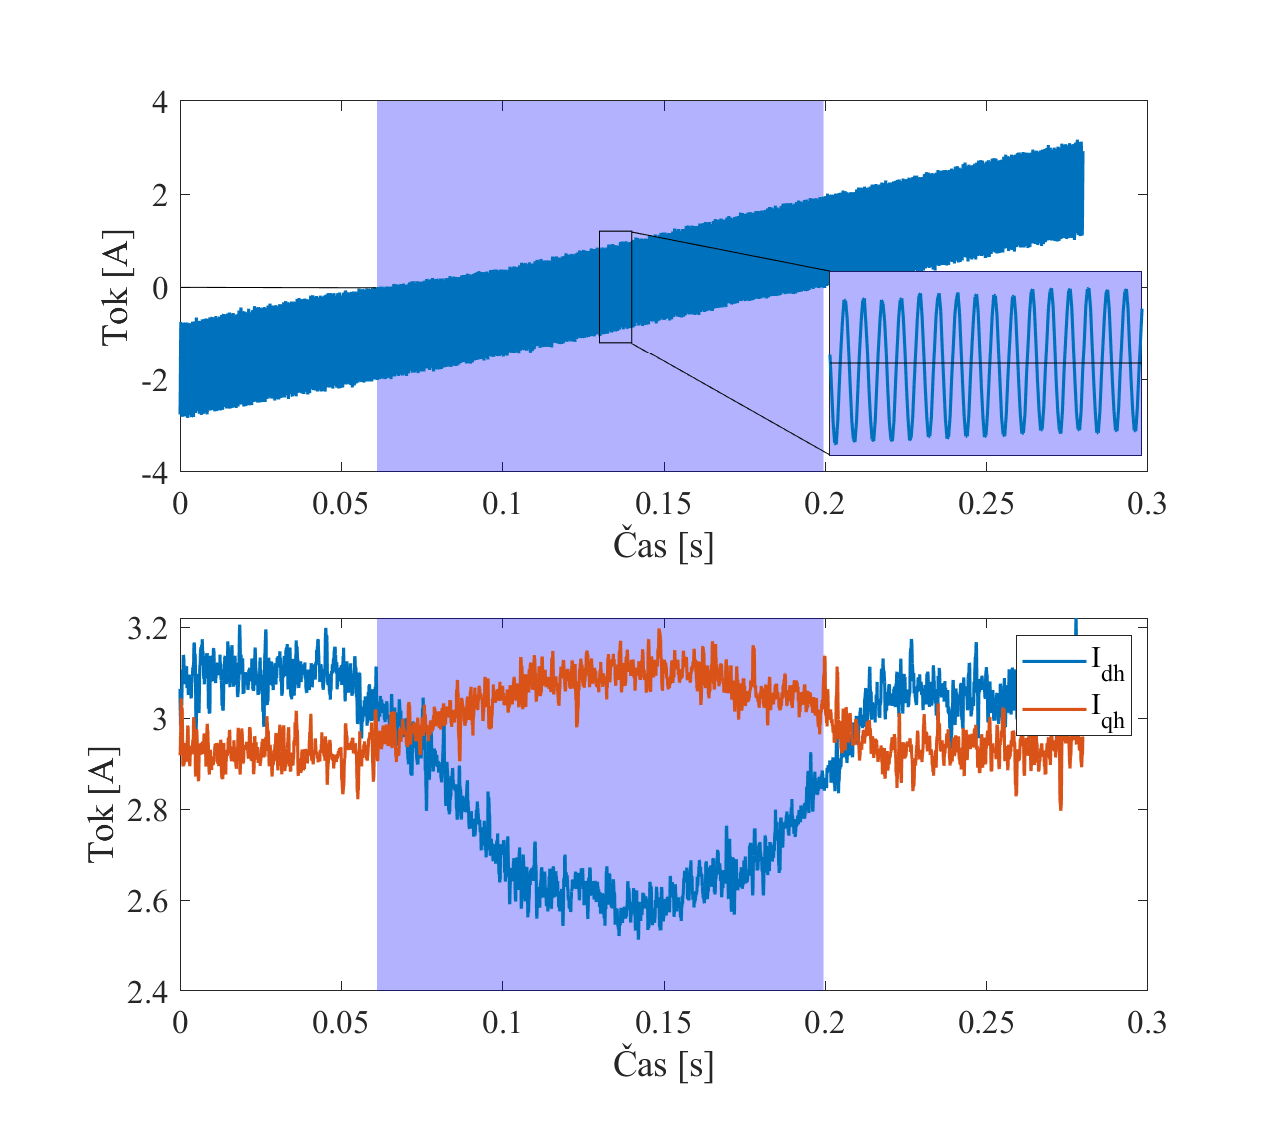
\includegraphics[width=1\columnwidth]{Slike/mrtviCasFazniTok.eps}
    \caption{\label{mrtviCasFazniTok} Vpliv mrtvega časa na faznem toku }
\end{figure}

Iz slike \ref{mrtviCasFazniTok} lahko sklepamo, da bo popačenje zaradi mrtvega časa večje tudi z večjo povprečno amplitudo VF tokovnega odziva (oziroma bo vidno v širšem kotu) in večje, če bo enosmerna
komponenta toka v FKS manjša, saj bo v večih kotnih pozicijah VF tokovna komponenta prehajala čez ničti tok, oziroma menjala polariteto. To lahko pokažemo z meritvami, prikazanimi na slikah
\ref{tokovniOdzivIs_HKSslediRKS_IdAmp_DT} in \ref{tokovniOdzivIs_HKSslediRKS_IqAmp_DT}, kjer je prikazana amplituda v vzdolžni in prečni smeri, in na sliki
\ref{tokovniOdzivIs_HKSslediRKS_IdiffAmp_DT}, kjer je prikazana njuna razlika.

\begin{figure}[!htbp]
    \centering
    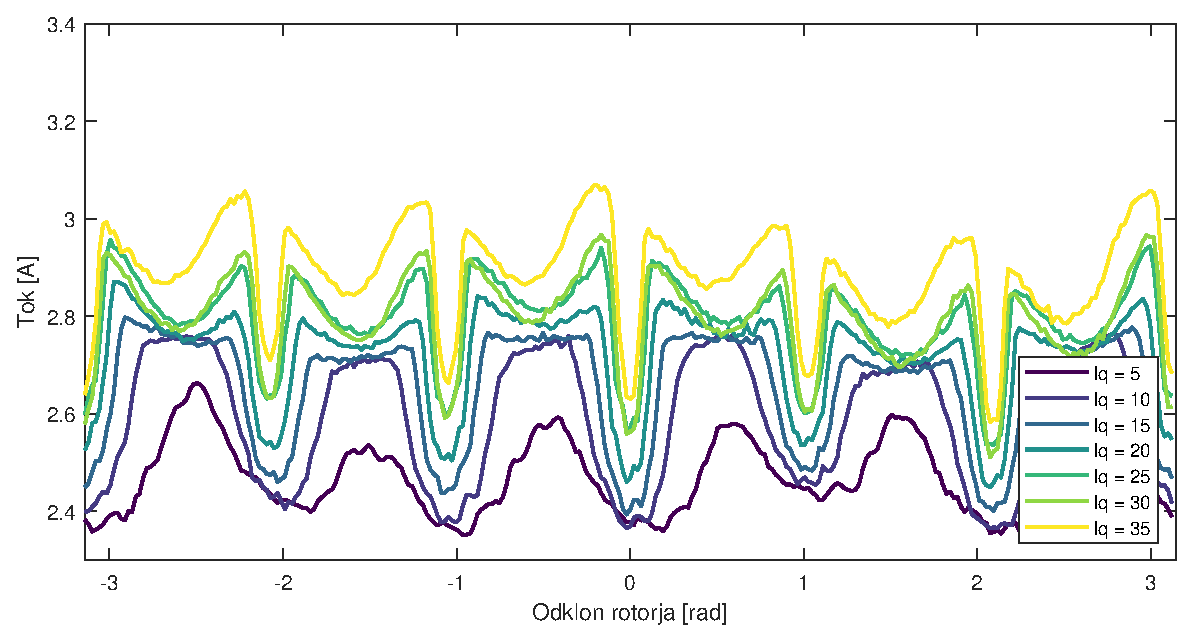
\includegraphics[width=0.75\columnwidth]{Slike/tokovniOdzivIs_HKSslediRKS_IdAmp_DT.eps}
    \caption{\label{tokovniOdzivIs_HKSslediRKS_IdAmp_DT} Vpliv prečnega toka na popačenje $\hat{i}_{dh}$ zaradi mrtvega časa. }
\end{figure}

\begin{figure}[!htbp]
    \centering
    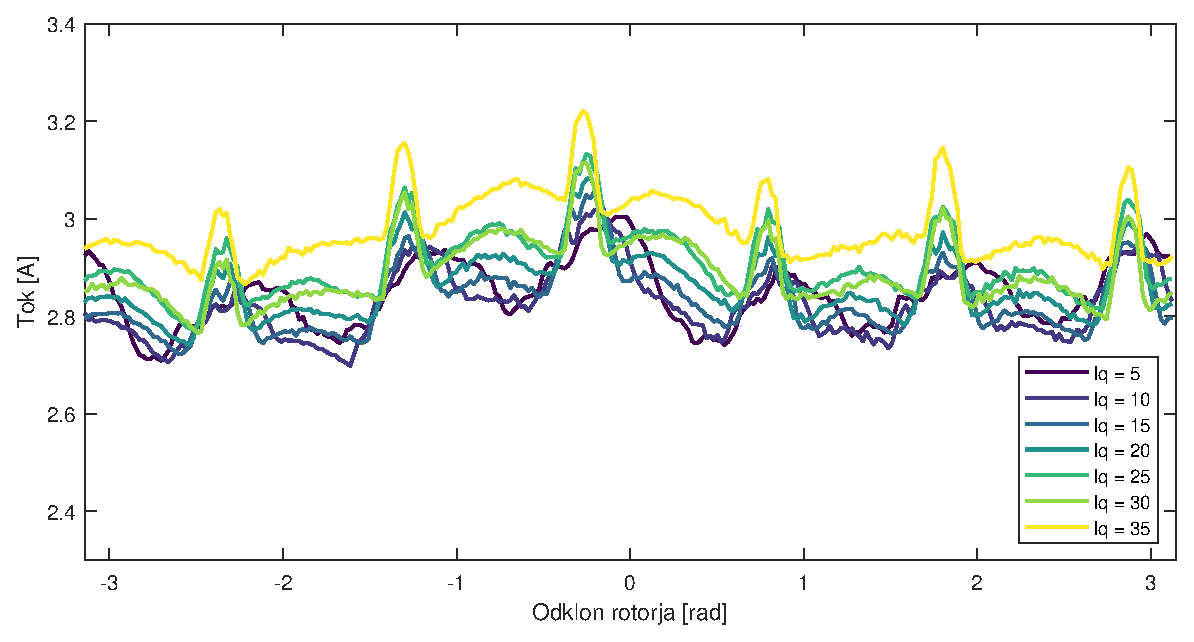
\includegraphics[width=0.75\columnwidth]{Slike/tokovniOdzivIs_HKSslediRKS_IqAmp_DT.eps}
    \caption{\label{tokovniOdzivIs_HKSslediRKS_IqAmp_DT} Vpliv prečnega toka na popačenje $\hat{i}_{qh}$ zaradi mrtvega časa. }
\end{figure}

\begin{figure}[!htbp]
    \centering
    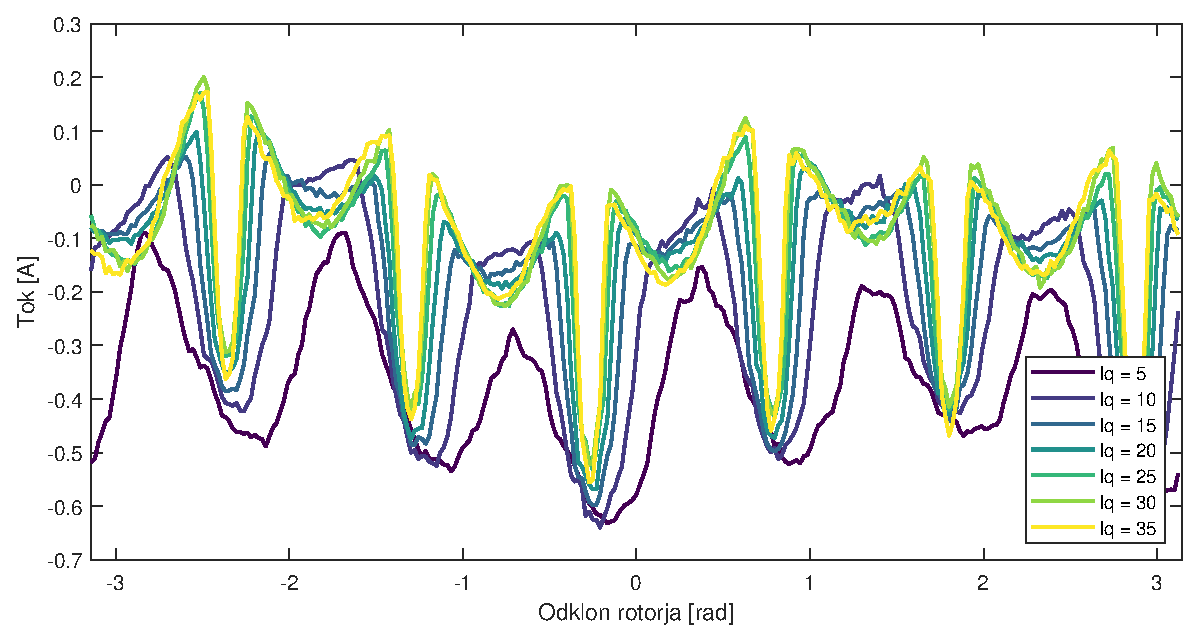
\includegraphics[width=0.75\columnwidth]{Slike/tokovniOdzivIs_HKSslediRKS_IdiffAmp_DT.eps}
    \caption{\label{tokovniOdzivIs_HKSslediRKS_IdiffAmp_DT} Vpliv prečnega toka na popačenje $\hat{i}_{e}$ zaradi mrtvega časa. }
\end{figure}


Takšno popačenje amplitude odziva naravno vpliva na oceno pozicije, saj bo PI regulator poiskušal zmanjšati napako in to tako, da bo spremenil odklon HKS na mesto, kjer imata odziva enako vrednost.
Sklepamo lahko tudi, da bo z višjimi tokovi napaka ocenejene pozicije manjša, saj se bo PI regulator zreguliral z manjšim odklonom, saj so motnje po kotu ožje. Vpliv mrtvega časa na oceno pozicije pa
je prikazan v zadnjem poglavju.

%================================================================================
%================================================================================
%**                             Integracija v FOC                           
%================================================================================
%================================================================================
\chapter{Integracija v FOC} \label{integracija}

Za uspešno implementacijo HFSI algoritma, ga je potrebno tudi pravilno integrirati v celotno FOC vodenje. Potrebno je poskrbeti za pravilno inicializacijo algoritma, filtriranje tokovne povratne
zanke, zadnji element pa je preklop v delovanje opazovalnika, ko vrtilna hitrost doseže dovolj visoko vrednost. Na koncu je predstavljen postopek uglaševanja PI regulatorja.

\section{Inicializacija HFSI}

Ker s HFSI algoritmom nismo zmožni ocenjevati polaritete rotorja, potrebujemo za pravilno smer vrtenja poskrbeti, da je začetna pozicija znana. Pred zagonom HFSI zaznamo začetno pozicijo rotorja, ki
se začne uporabljati že od samega začetka delovanja HFSI. Ker je HKS od RKS odklonjen za $\frac{\pi}{4}$, je začetna vrednost kota HKS enaka ocenjeni začetni vrednosti RKS z odklonom $\frac{\pi}{4}$.
\\
Pri delovanju HFSI tokovna povratna zanka vključuje tudi VF komponento, ki jo je potrebno izfiltrirati, saj lahko regulatorja toka s povratno zanko vplivata na VF odziv ali pa celo destabilizirata
sistem. Uporabimo zaporni pasovni filter (BSF). Filtriranja ne smemo izvesti v SKS, saj je tam VF komponenta različne frekvence, ki je odvisna tudi od vrtilne hitrosti HKS. Zato filtriramo v FKS, kjer
ima konstantno frekvenco in sicer enako vzbujalnem signalu. Ker filtriramo v FKS, pa lahko filtrirane tokove $i_d$ in $i_q$ direktno uporabimo za regulacijo toka. Ob zagonu prvih nekaj period
vzbujalnega signala FOC regulatorje izklopimo, da se prehodni pojav pasovnih filtrov ustali. 

% profesor: Bi bilo tukaj smiselno dodati še sliko filtriranja povratne tokovne zanke?

\section{Začetni kot in izbira stabilne delovne točke}

Ob inicializaciji HFSI algoritma, moramo določiti začetno pozicijo in tako primerno tudi postaviti HKS v stabilno točko regulacije - do sedaj smo vedno definirali to točko kot odklon od RKS za
$\frac{\pi}{4}$. Smo pa že pri matematičnem zapisu tokovnih odzivov in tudi realnih odzivov opazili, da so štiri stabilne regulacijske točke - torej tisti odkloni HKS od RKS, kjer ima razlika amplitudnih
odzivov ali regulirana veličina vrednost nič. Tako bi pričakovali, da je lahko tudi odklon HKS od RKS poljuben, oziroma bolj točno $\frac{\pi}{4} + k\frac{\pi}{2}$, kjer je k poljubno naravno število.
Nato pa smo pokazali z meritvijo, prikazano na sliki \ref{reguliranaVelicinaIs}, da se regulirana veličina okoli stabilnih točk pri višjih prečnih tokovih obnaša drugače. V dveh točkah je linearna, v
drugih dveh pa ima v eni smeri drugačen naklon kot v drugi. Torej bi pričakovali, da bi dobili tudi drugačno obnašanje algoritma v različnih točkah, vendar pa se je izkazalo, da algoritem ni tako
občutljiv in niti ni važno v katero začetno stabilno točko ga postavimo (četudi ga v končni implementaciji vedno postavimo v stabilno točko, ki ima najbolj linearno okolico). Tukaj moramo paziti, da
ne ustvarimo pozitivne povratne zanke s postavitvijo v napačno začetno stabilno točko. HKS lahko postavimo v katerokoli od štirih obstoječih, vendar ima regulirana veličina okoli dveh pozitiven
naklon, okoli drugih dveh pa negativen. Če ne spremenimo predznaka regulirane veličine v dveh stabilnih točkah, kjer ima ta negativen naklon bo nastala pozitivna povratna zanka, ki destabilizira
sistem.

\section{Brezudarni preklop v delovanje opazovalnika}

Proti koncu delovanja HFSI algoritma, ko je vrtilna hitrost že dovolj visoka, da ocenjujemo pozicijo rotorja z inducirano napetostjo, je potrebno izvesti brezudarni preklop. Takoj po preklopu želimo,
da opazovalnik začne delovati v pravilni delovni točki. To lahko dosežemo tako, da opazovalnik deluje že pred preklopom, vzporedno s HFSI algoritmom. Ob preklopu tako samo izklopimo vzbujanje
statorja. Ta način pa terja dodatne kalkulacije, ki so lahko v določenih sistemih, kjer je nadvsem pomembna nizka cena in zato uporaba manj zmogljivih procesorjev, previsoke. Zato se uporabi drug
način, ki pa ob preklopu postavi opazovalnik v željeno delovno točko. To pomeni, da je potrebno vsa notranja stanja postaviti na pravilno začetno vrednost. To vključuje notranja stanja modela, ki se
uporabljajo za ocenjevanje inducirane napetosti, ocenjeno hitrost in pozicijo. Problem pri tej metodi pa je, da se je težko izogniti manjšim prenihajem, saj bo vedno prisotna napaka ocene
pozicije in hitrosti algoritma HFSI in ima zato opazovalnik ob preklopu že neko majhno napako. Na sliki \ref{brezudarniPreklop} sta na prvem grafu prikazani ocenjeni hitrosti HFSI algoritma in
opazovalnika. Ob preklopu, ki se zgodi okoli 0.5 sekunde, hitrost opazovalnika predpolnimo z ocenjeno hitrostjo HFSI algoritma. Drugi graf prikazuje ocenjeno pozicijo obeh algoritmov, na zadnjem grafu
pa je prikazana napaka ocenjenega kota. Po preklopu se opazi minimalen prenihaj.

\begin{figure}[!htbp]
    \centering
    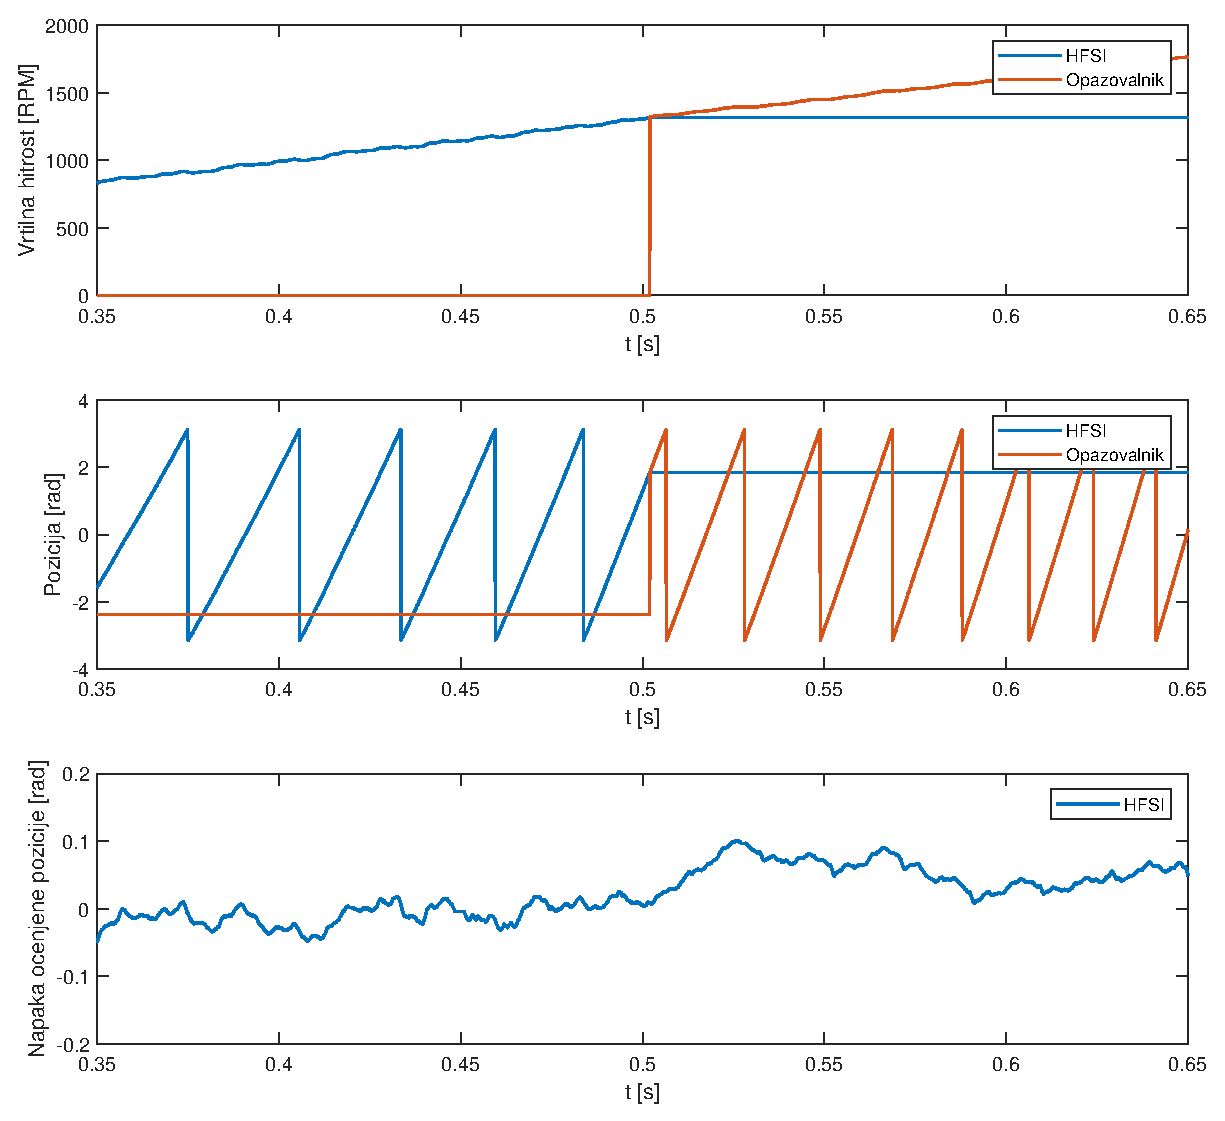
\includegraphics[width=1\columnwidth]{Slike/brezudarniPreklop.eps}
    \caption{\label{brezudarniPreklop} Preklop v delovanje opazovalnika pozicije. }
\end{figure}

\section{Nastavitev parametrov PI regulatorja}

Parametri regulatorja so bili nastavljeni ročno in sicer z opazovanjem delovanja algoritma pri različnih parametrih. Za kriterijsko funkcijo smo izbrali napako ocenjenega kota in je bila najprej
pomerjena pri desetih različnih $K_p$ parametrih, kjer je imel parameter $K_i$ neko začetno vrednost, pri kateri je bil algoritem stabilen. Nato se je izbral $K_p$ z najmanjšo napako in ponovno pomeril
odziv s tem parametrom in različnimi $K_i$ parametri. Tako smo pridobili $K_p$ in $K_i$ s prvo iteracijo, nato pa se izvedla dodatna iteracija, da smo prišli do optimalnih parametrov. 
\\
V prvi iteraciji je bil obseg vrednosti parametrov, pri katerij se je meril odziv tak, da je algoritem pri robnih vrednostih postal nestabilen. Ko se je izvajala druga iteracija pa se je obseg
parametrov zmanjšal in je bil okoli vrednosti, pridobljene s prvo iteracijo.
\\
Na slikah \ref{PItuning_Kp_unstableLow} - \ref{PItuning_Kp_stable} so prikazani vplivi napačne izbire $K_p$ parametra. Premajhen parameter povzroči večinoma integralski odziv in dobimo velike dolge
prenihaje, prevelik pa popolnoma destabilizira sistem. Zadnja slika prikazuje optimalno izbiro, kjer ocenjena pozicija sledi dejanski brez večje napake.
\begin{figure}[!htbp]
    \centering
    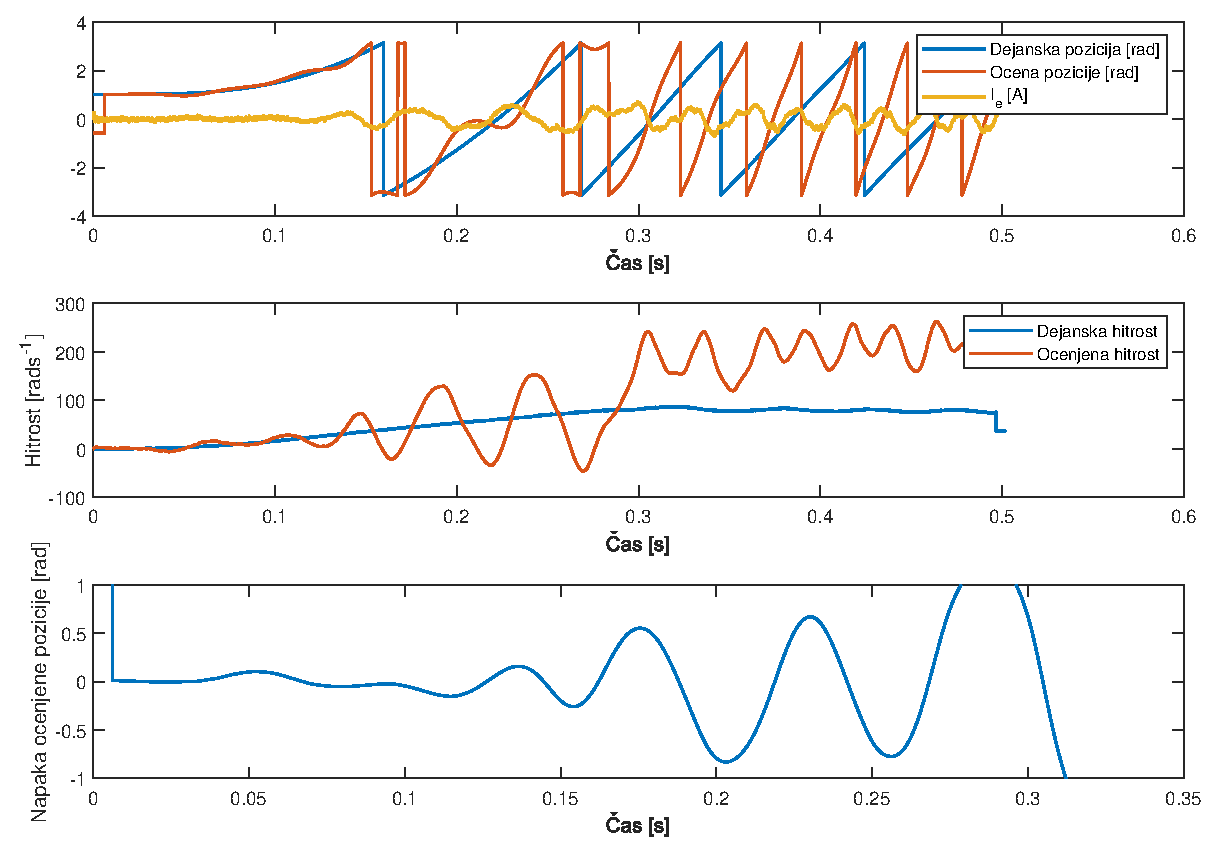
\includegraphics[width=0.75\columnwidth]{Slike/PItuning_Kp_unstableLow.eps}
    \caption{\label{PItuning_Kp_unstableLow} Prikaz vpliva premajhnega $K_p$ parametra. }
\end{figure}

\begin{figure}[!htbp]
    \centering
    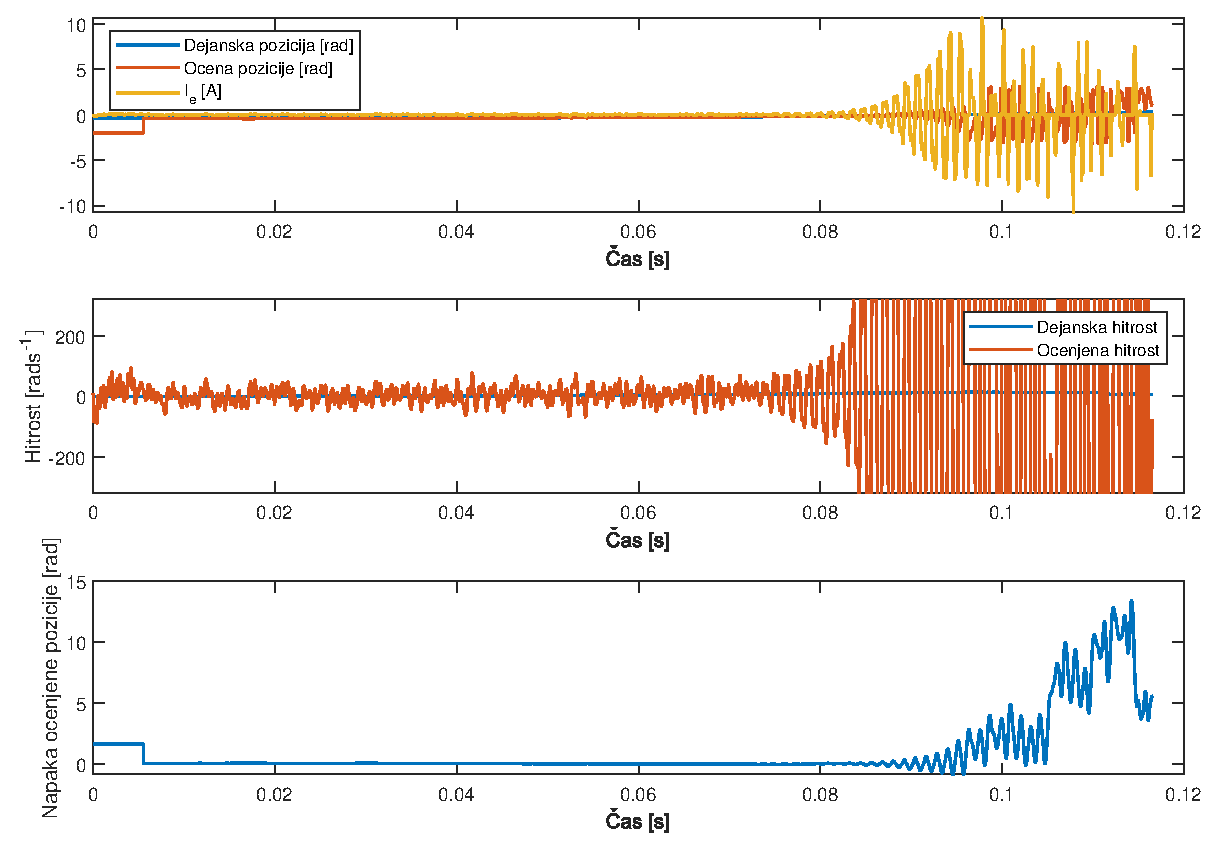
\includegraphics[width=0.75\columnwidth]{Slike/PItuning_Kp_unstableHigh.eps}
    \caption{\label{PItuning_Kp_unstableHigh} Prikaz vpliva prevelikega $K_p$ parametra. }
\end{figure}

\begin{figure}[!htbp]
    \centering
    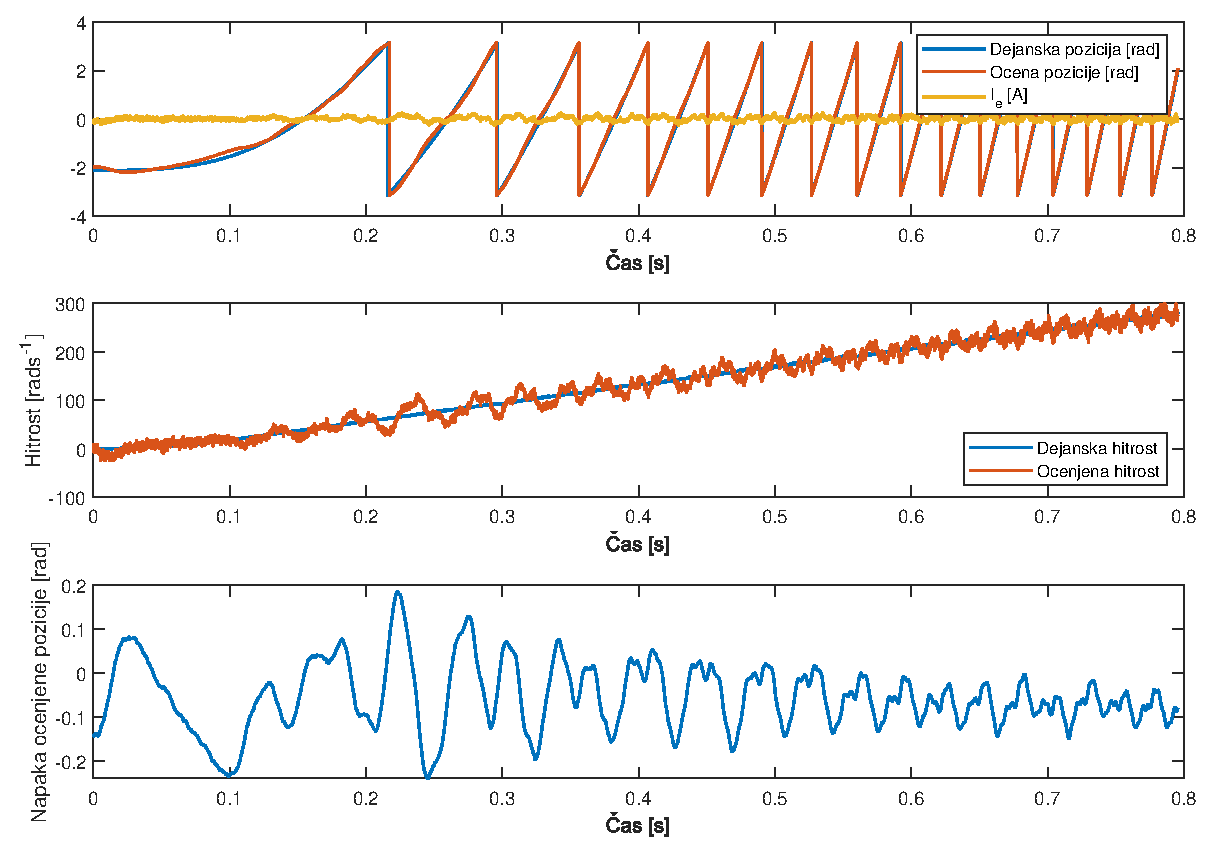
\includegraphics[width=0.75\columnwidth]{Slike/PItuning_Kp_stable.eps}
    \caption{\label{PItuning_Kp_stable} Prikaz vpliva optimalnega $K_p$ parametra. }
\end{figure}

Slike \ref{PItuning_Ki_unstableLow} - \ref{PItuning_Ki_stable} pa prikazujejo vpliv $K_i$ parametra. Z izbiro premajhnega parametra regulirno veličino nikoli ne zreguliramo na nič, kar povzroči
konstantno napako. Brez uporabe $K_i$ parametra pa stroj pade iz sinhronizacije. Prebelik $K_i$ ponovno destabilizira sistem, opzimalen z optimalnim parametrom pa dobimo podoben odziv kot na sliki 
\ref{PItuning_Kp_stable}, saj je bil $K_p$ parameter že optimalno izbran.

\begin{figure}[!htbp]
    \centering
    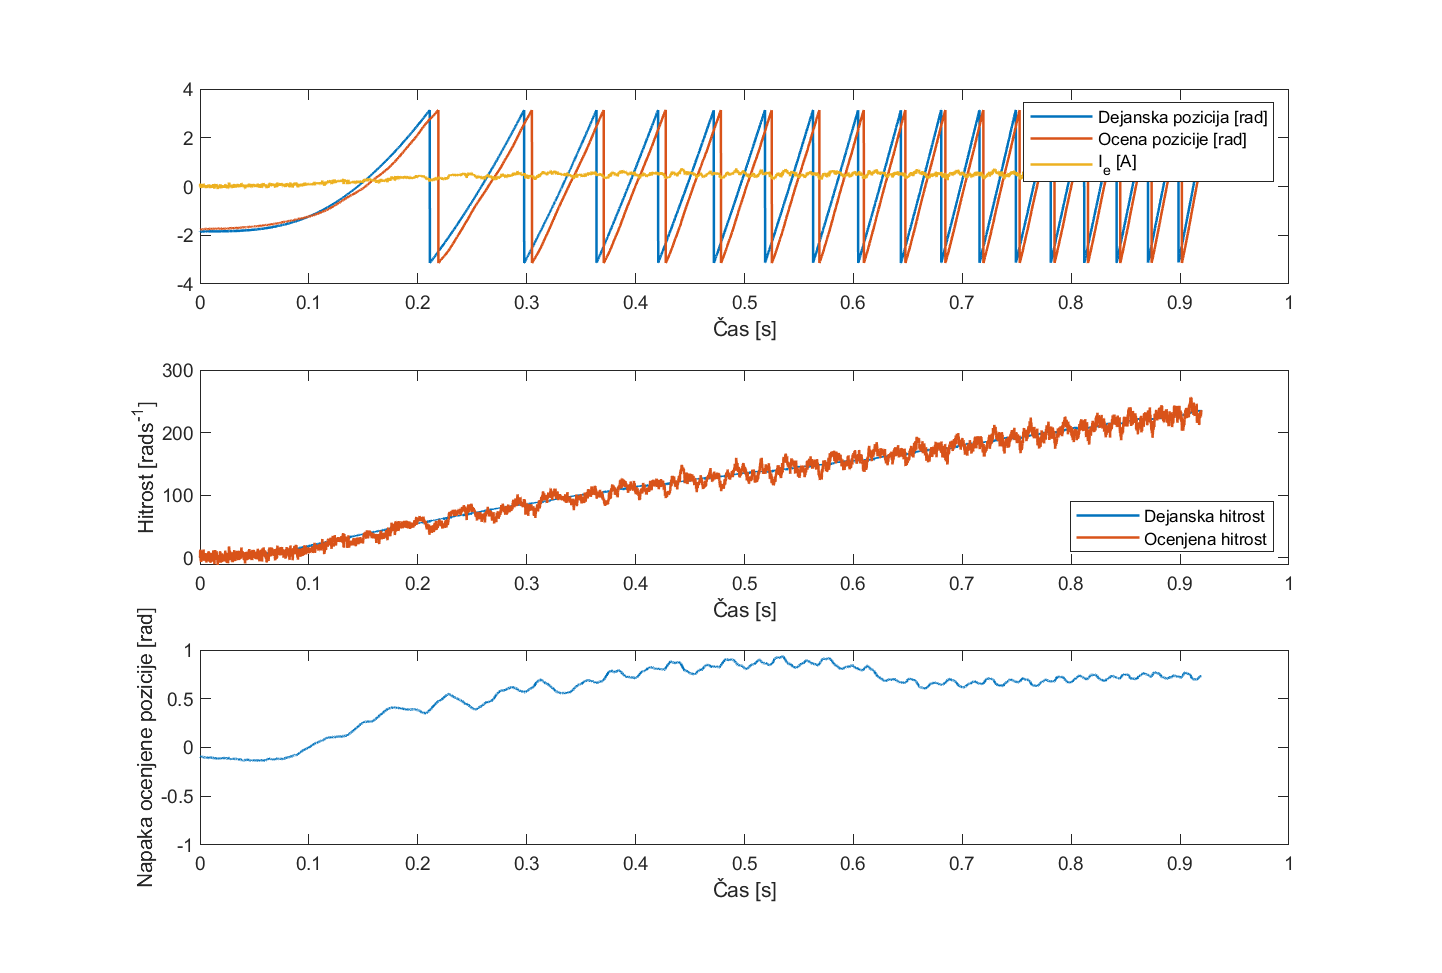
\includegraphics[width=0.75\columnwidth]{Slike/PItuning_Ki_unstableLow.eps}
    \caption{\label{PItuning_Ki_unstableLow} Prikaz vpliva premajhnega $K_i$ parametra. }
\end{figure}

\begin{figure}[!htbp]
    \centering
    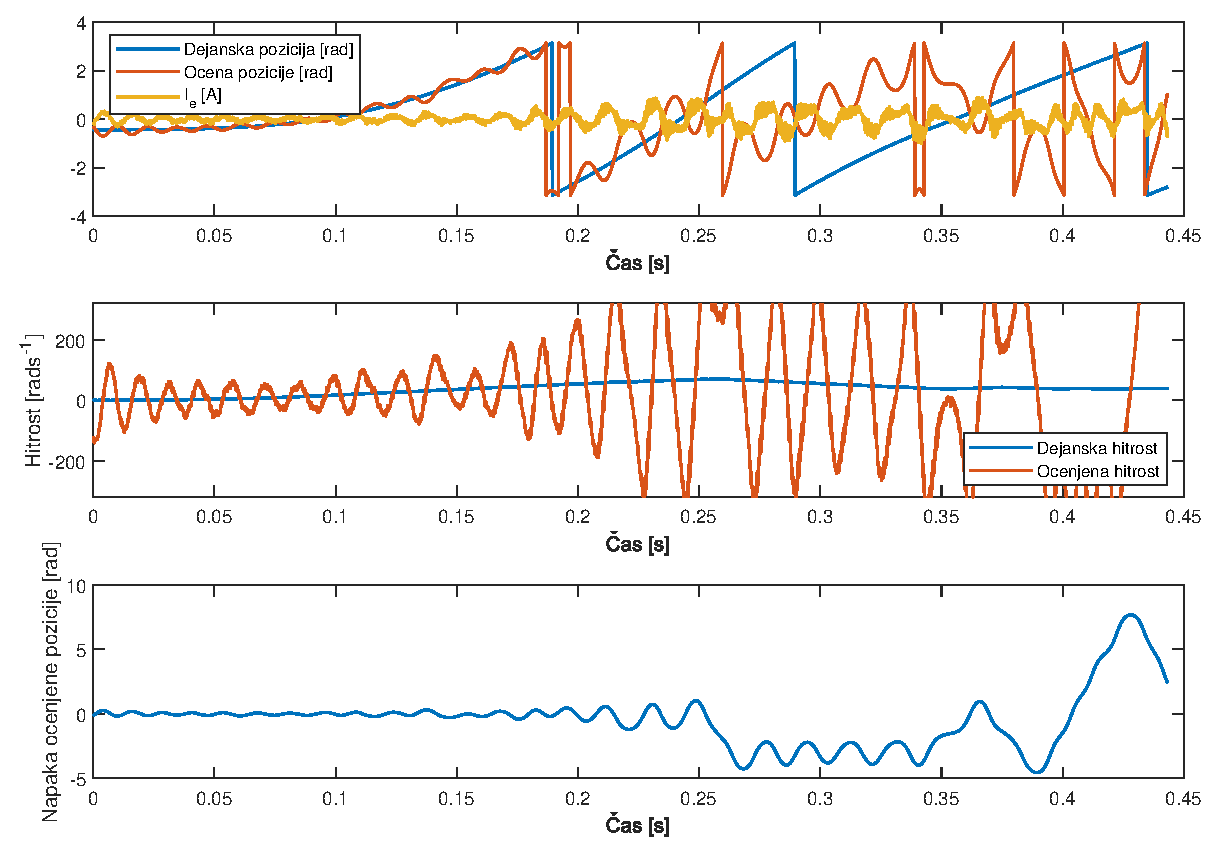
\includegraphics[width=0.75\columnwidth]{Slike/PItuning_Ki_unstableHigh.eps}
    \caption{\label{PItuning_Ki_unstableHigh} Prikaz vpliva prevelikega $K_i$ parametra. }
\end{figure}

\begin{figure}[!htbp]
    \centering
    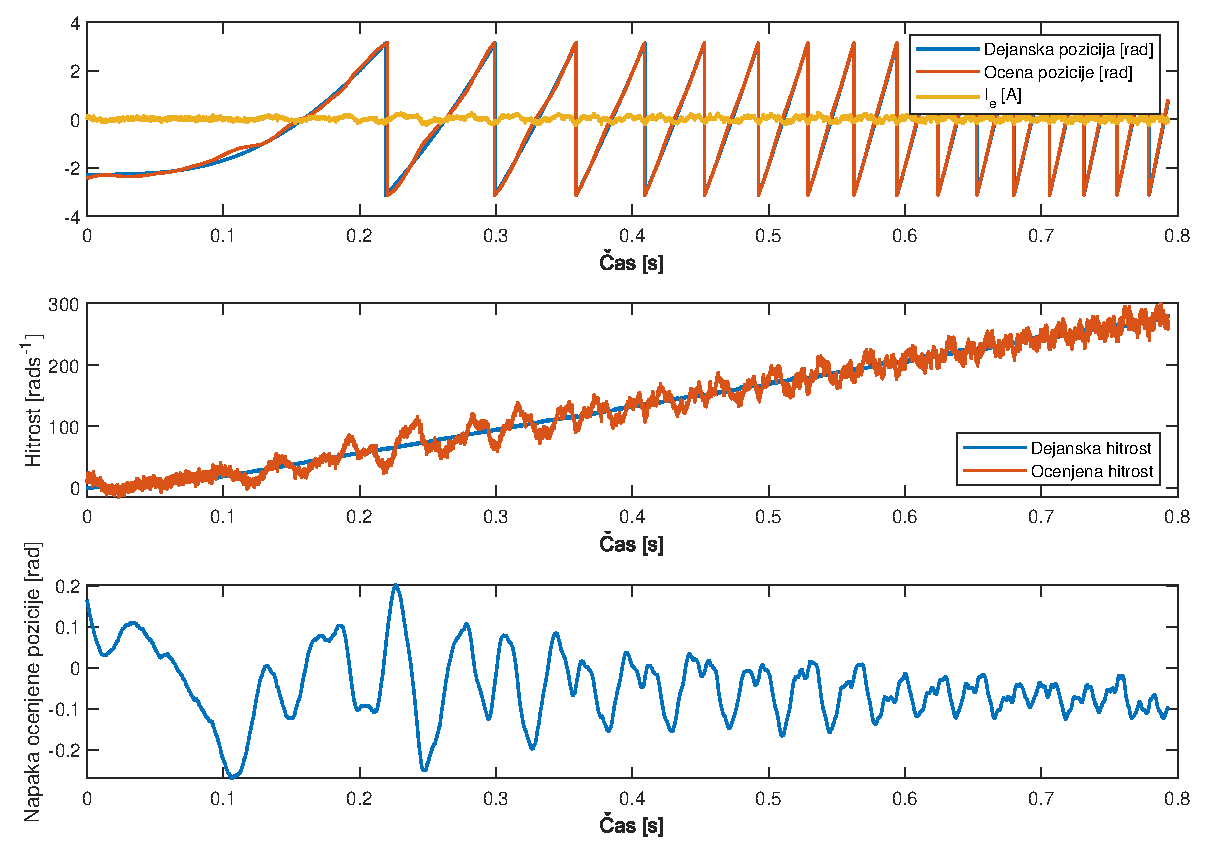
\includegraphics[width=0.75\columnwidth]{Slike/PItuning_Ki_stable.eps}
    \caption{\label{PItuning_Ki_stable} Prikaz vpliva optimalnega $K_i$ parametra. }
\end{figure}


\chapter{Eksperimenti}  \label{eksperimenti}

V tem poglavju je najprej opisano krmiljenje napetostnega pretvornika in merjenje toka, saj tudi to vpliva na algoritem. Na koncu so prikazane meritve realnega sistema, ki so bile zajete z
osciloskopom, interne spremenljivke, uporabljene v samem algoritmu, pa so bile v realnem času poslane na računalnik preko serijske komunikacije.

\begin{figure}[!htbp]
    \centering
    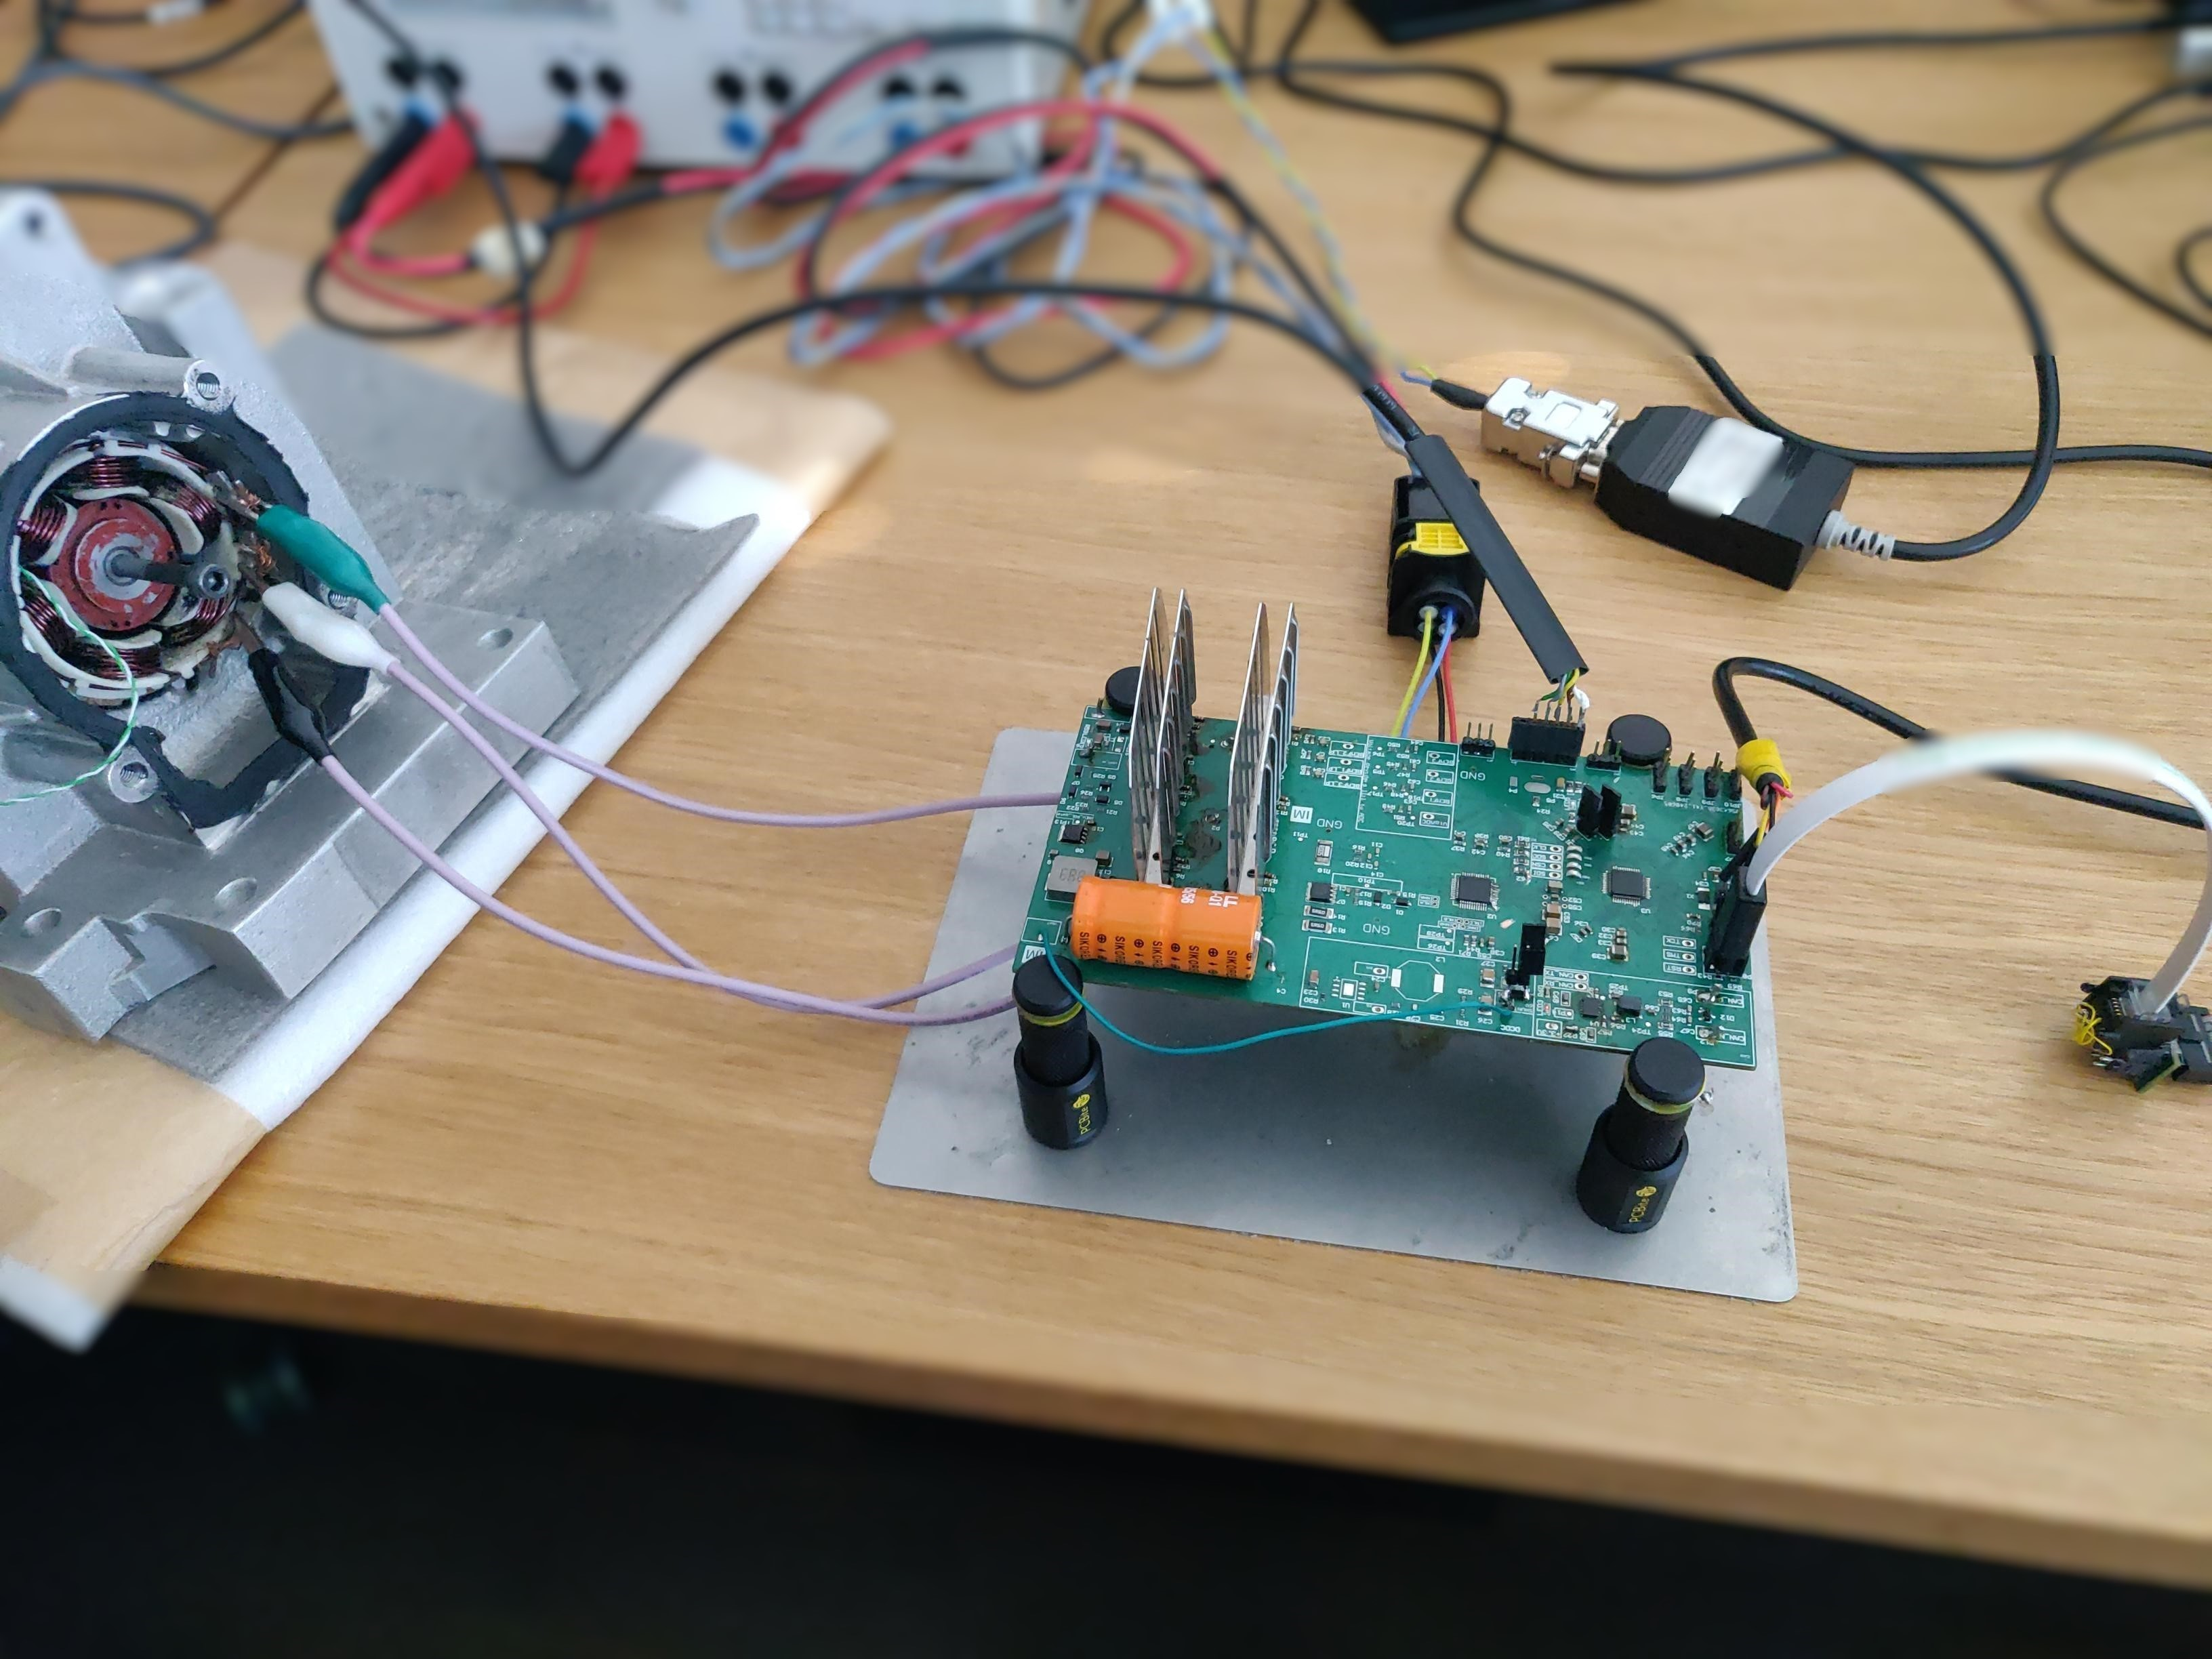
\includegraphics[width=0.75\columnwidth]{Slike/EksperimentiSlika.jpg}
    \caption{\label{experimentiSlika} Fotografija močnostnega pretvornika in stroja}
\end{figure}

Na fotografiji \ref{experimentiSlika} je prikazan sistem, na katerem je bil razvit HFSI algoritem. 

\section{Trifazni PWM in meritev toka}

V sistemu se uporablja asimetričen PWM s fazno zamaknjenimi fazami. Največja prednost tega je preprosta implementacija krmiljenja napetosti in merjenje toka, slaba lastnost pa je večje valovanje
frekvence PWM-ja. Potek faznih napetosti je prikazan na sliki \ref{PWM}, kjer se vidi fazni zamak faz - fazno sta zamaknjeni druga in tretja faza za merjenje toka. $t_{PWM}$ je perioda PWM, $t_{MEAS}$
pa je časovni zamik poteka faze za tokovno meritev. $t_0$ do $t_5$ pa so časi, kjer faze spremenijo polariteto. Ti časi določajo, kakšna je efektivna napetost na fazah in se izračunajo kot je
prikazano z enačbo \ref{izracunPWM}. $t_0$, $t_1$ in $t_2$ se ne spreminjajo, saj takrat merimo tok, $t_3$, $t_4$ in $t_5$ pa so odvisni od željenih faznih napetosti. Implementacija na mikrokrmilniku
potrebuje še dodatno pretvorbo iz časa v število taktov PWM periferije krmilnika.

\begin{figure}[!htbp]
    \centering
    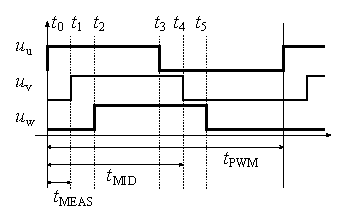
\includegraphics[width=1\columnwidth]{Slike/Inkscape/PWM.eps}
    \caption{\label{PWM} Pulzno širinska modulacija močnostnega pretvornika }
\end{figure}

\begin{equation} \label{izracunPWM}
\begin{gathered}
    t_0 = 0  \\
    t_1 = t_{MEAS}  \\
    t_2 = 2t_{MEAS}  \\
    t_3 = t_{MID} + u_uC  \\
    t_4 = t_{MID} + t_{MEAS} + u_vC \\
    t_5 = t_{MID} + 2t_{MEAS} + u_wC
\end{gathered}
\end{equation}

$t_{MID}$ ni polovica $t_{PWM}$, saj smo rezervirali $2t_{MEAS}$ periode za meritev toka. Zato je $t_{MID}$ enak polovici $t_{MID} - 2t_{MEAS}$. $C$ pa je faktor za pretvorbo željenje napetosti v
čas in je preprosto razmerje med dolžino periode in napetostno zalogo. Napetostna zaloga - oziroma napajalna napetost - se aktivno meri, saj želimo da je dejanska napetost na izhodu enaka željeni. Pri
FOC vodenju to praviloma ni problem, saj regulatorji toka to napako odpravijo. HFSI algoritem pa vsebuje tudi visokofrekvenčno napetostno vzbujanje in se predpostavlja, da je taka tudi na izhodu in ni
odvisna od napajalne napetosti. Če bi ta bila odvisna, bi pri višjih napajalnih napetostih dobili večji tokovni odziv, kar pa si lahko predstavljamo kot ojačanje povratne zanke - to pa bi sledilo v
spremembo dinamike regulacijskega sistema, ki ga HFSI vsebuje.

\begin{figure}[!htbp]
    \centering
    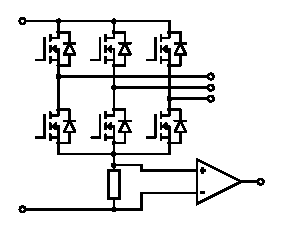
\includegraphics[width=0.5\columnwidth]{Slike/Inkscape/inverter.eps}
    \caption{\label{inverter} Shema močnostnega pretvornika in meritve toka }
\end{figure}

Na sliki \ref{inverter} je prikazan močnostni pretvornik, prav tako pa je prikazano merjenje toka. Uporabljena je konfiguracija enega shunta, kar pomeni, da ko bodo vse tri faze na napajalni
napetosti ali na 0V, skozi shunt ne bo tekel tok. Zato meritev delamo v začetku PWM periode, ko naprej preklopimo prvo fazo, nato pa drugo. Na sliki \ref{meritevTokaIu} je prikazana prva meritev.
Če definiramo tok, ki teče v stroj kot pozitiven tok, v tem času merimo tok $i_u$, saj teče iz prve faze v stroj, se porazdeli med drugo in tretjo fazo in skozi shunt. 

\begin{figure}[!htbp]
    \centering
    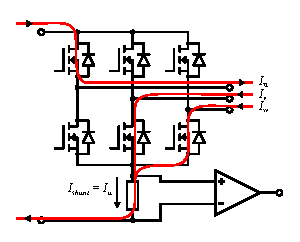
\includegraphics[width=0.5\columnwidth]{Slike/Inkscape/meritevTokaIu.eps}
    \caption{\label{meritevTokaIu} Meritev toka $i_u$ }
\end{figure}

Na sliki \ref{meritevTokaIw} pa je prikazana druga meritev, kjer tok steče skozi prvo in drugo fazo v stroj, iz tretje faze stroja pa skozi shunt, zato tukaj merimo negativen tok $i_w$. 

\begin{figure}[!htbp]
    \centering
    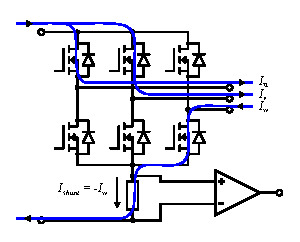
\includegraphics[width=0.5\columnwidth]{Slike/Inkscape/meritevTokaIw.eps}
    \caption{\label{meritevTokaIw} Meritev toka $-i_w$ }
\end{figure}

Tok druge faze $i_v$ pa izračunamo po enačbi \ref{izracunIv} iz dveh meritev, saj velja $i_u + i_v + i_w = 0$.

\begin{equation} \label{izracunIv}
i_v = -(i_u + i_w)
\end{equation}

Na sliki \ref{fazeInShunt} so prikazane vse tri fazne napetosti in izhod ojačevalnika.

\begin{figure}[!htbp]
    \centering
    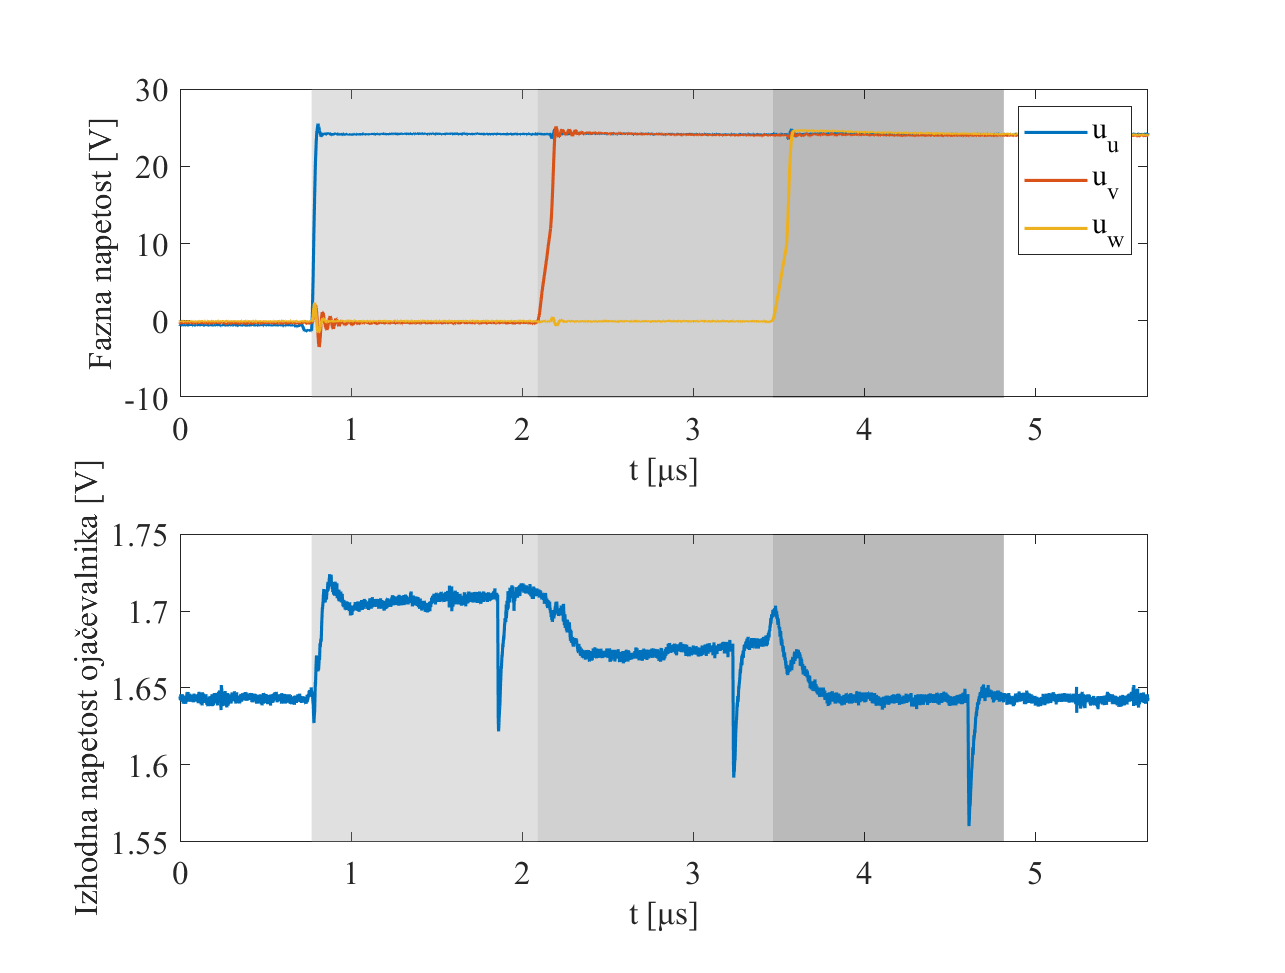
\includegraphics[width=0.75\columnwidth]{Slike/fazeInShunt.eps}
    \caption{\label{fazeInShunt} Fazne napetosti in ojačan signal shunta. }
\end{figure}


\section{Rezultati} \label{rezultati}

V času razvoja algoritma je bilo opaženo, da se ta različno obnaša, ko hitro pospeši do končne hitrosti brez povečanega bremenskega navora in ko je bremenski navor visok, oziroma če ga vrtimo zelo
počasi. Na sliki \ref{NoLoadRun} je prikazano delovanje algoritma in ocena pozicije brez dodatnega bremenskega navora. Na sliki \ref{HighLoadRun} pa je bila pozicija rotorju vsiljena tako, da smo ga
vrteli s hitrostjo enega obrata na 10 sekund.

\begin{figure}[!htbp]
    \centering
    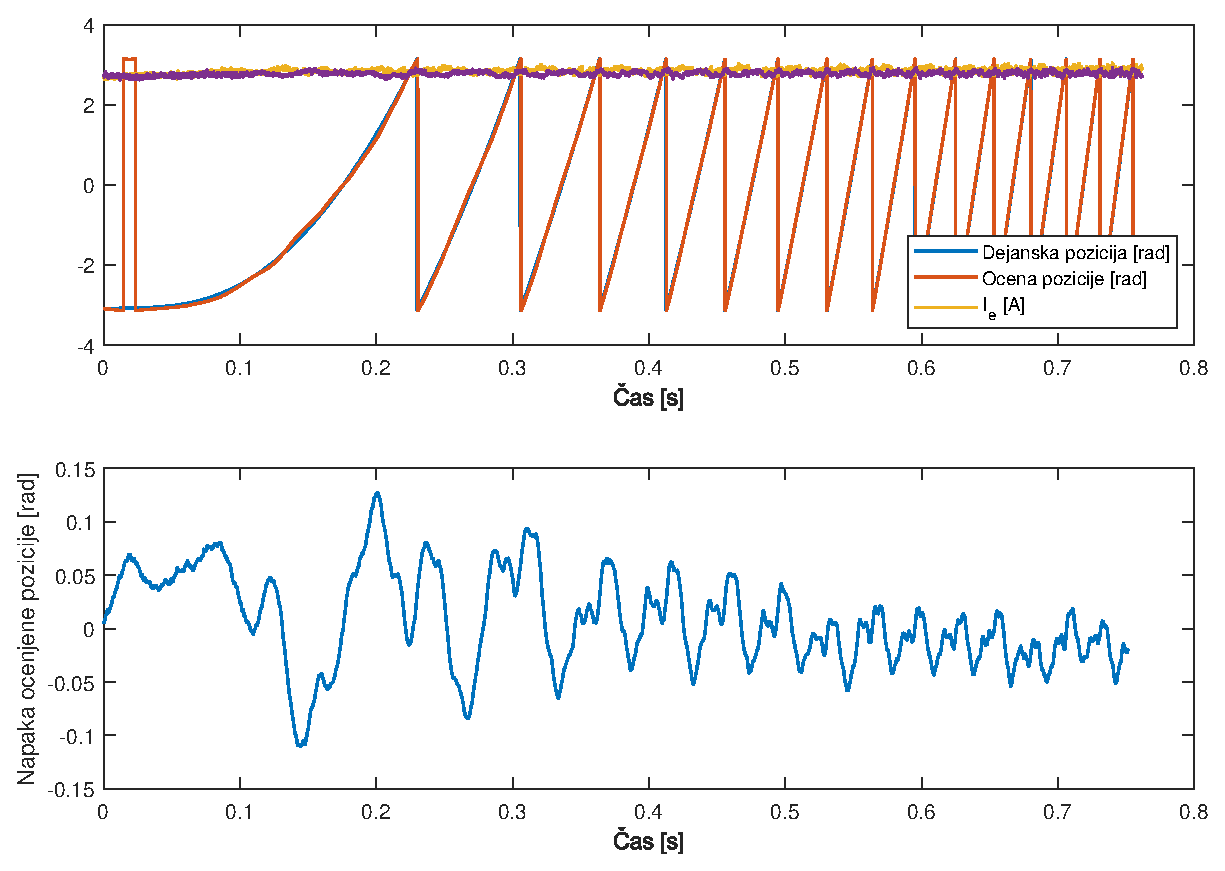
\includegraphics[width=0.8\columnwidth]{Slike/NoLoadRun.eps}
    \caption{\label{NoLoadRun} Ocena pozicije rotorja brez dodatnega bremena. }
\end{figure}

\begin{figure}[!htbp]
    \centering
    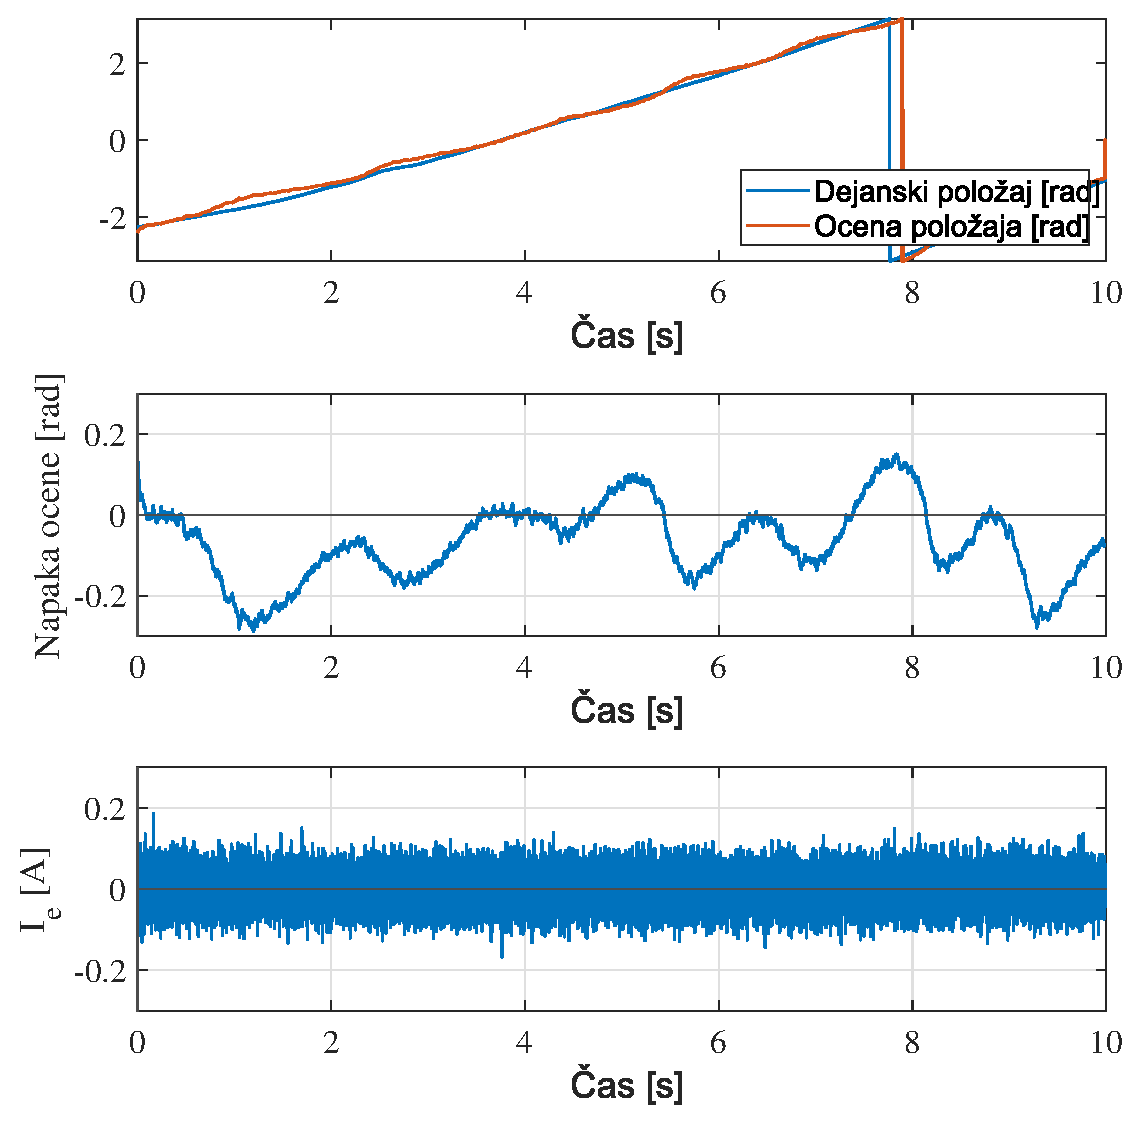
\includegraphics[width=0.8\columnwidth]{Slike/HighLoadRun.eps}
    \caption{\label{HighLoadRun} Ocena pozicije rotorja pri zelo nizkih hitrostih. }
\end{figure}

Na prvi sliki opazimo, da brez dodatne obremenitve stroj hitro pospeši in vztrajnost integratorja poskrbi, da se z oceno pozicije ne ujamemo v razne napake odziva zaradi mrtvega časa ali drugih
pojavov. Se pa ti opazijo na amplitudi VF tokovnih odzivov kot višjeharmonsko valovanje. Ko pa vrtimo stroj z nizko hitrostjo, regulator bolje zregulira razliko amplitud, vendar pa je zaradi pojavov
omenjenih v poglavju \ref{teorija} napaka ocene pozicije večja.

Na koncu tega poglavja smo prav tako pokazali vpliv prečnega toka na tokovni odziv, kjer je bilo opaziti višje harmonsko komponento, ki nam je kvarila odziv in je bila višja z višjim tokom. To se pozna
tudi na oceni kota, kot je prikazano na slikah \ref{vsiljenaPozicijaTokovi_angle} in \ref{vsiljenaPozicijaTokovi_angleError}. Opazimo, da je napaka pri nižjih tokovnih majhna in relativno
nespremenljiva, z višjimi tokovih pa postane večja. 

\begin{figure}[!htbp]
    \centering
    \includegraphics[width=0.8\columnwidth]{Slike/vsiljenaPozicijaTokovi_angle.eps}
    \caption{\label{vsiljenaPozicijaTokovi_angle} Ocena kota pri različnih prečnih tokovih. }
\end{figure}

\begin{figure}[!htbp]
    \centering
    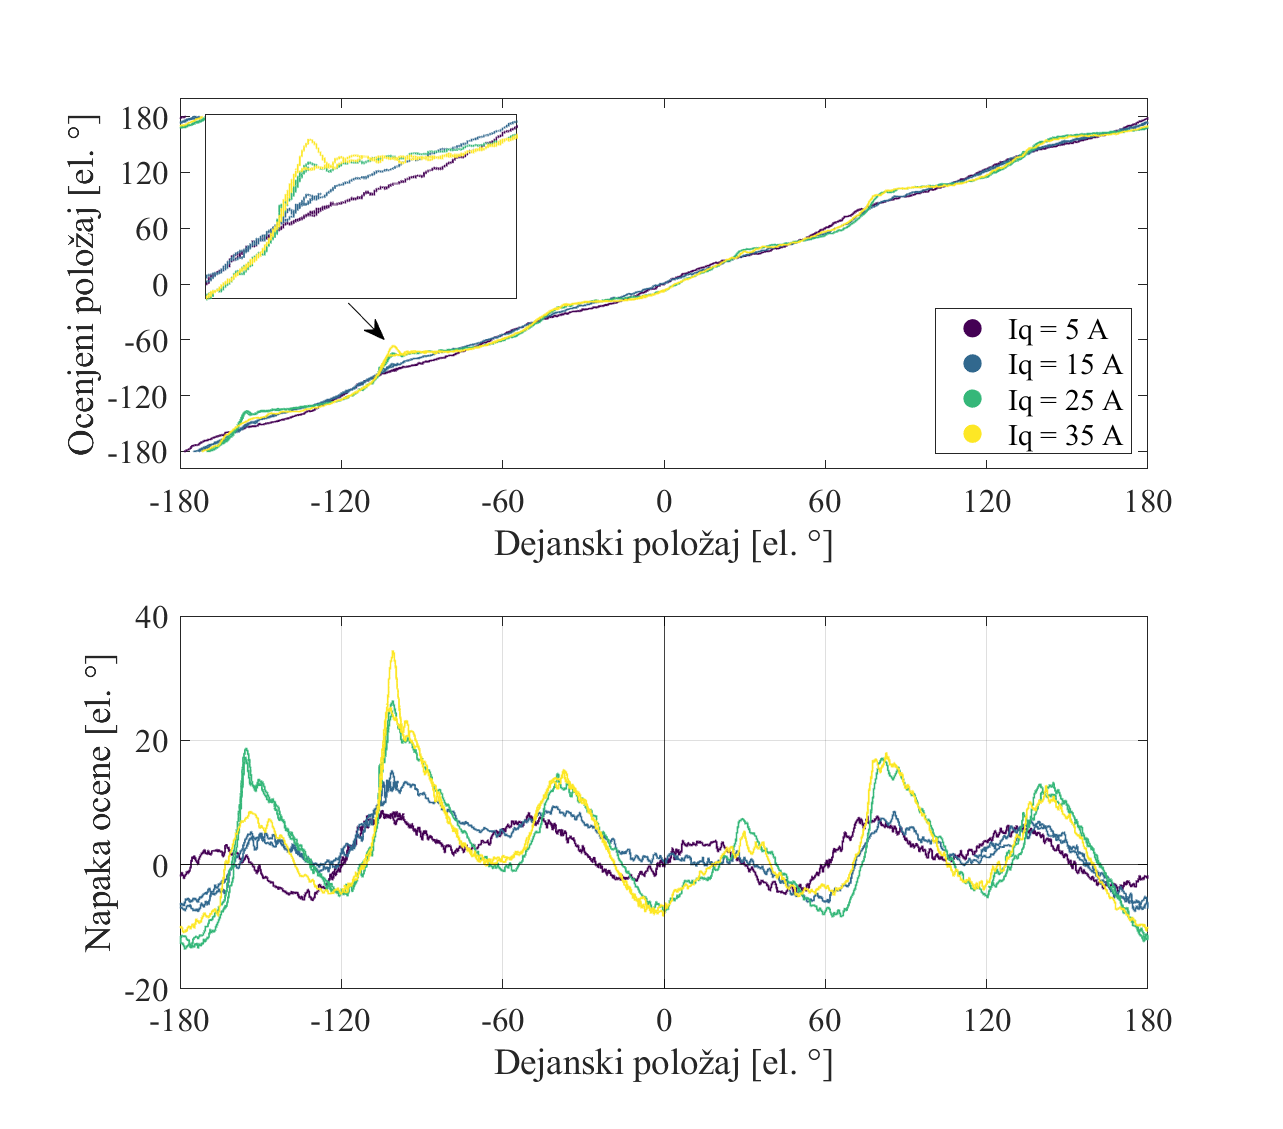
\includegraphics[width=1.0\columnwidth]{Slike/vsiljenaPozicijaTokovi_angleError.eps}
    \caption{\label{vsiljenaPozicijaTokovi_angleError} Napaka ocene kota pri različnih prečnih tokovih. }
\end{figure}

Poglejmo še vpliv mrtvega časa - pokazali smo da ima ta vpliv na tokovni odziv, ki je v času efekta mrtvega časa močno popačen. Na slikah \ref{vsiljenaPozicijaMrtviCasPlot_angle} in
\ref{vsiljenaPozicijaMrtviCasPlot_angleError} je prikazan vpliv mrtvega časa na oceni pozicije. Vidimo, da imamo ostre prehode, na pozicijah $k\frac{pi}{3}$, kar je ravno takrat, ko smo poravnani s
fazami oziroma, ko s faznimi tokovi preidemo čez nič. Prečni tok pri tem eksperimentu je bil nominalen (18 A). Lahko pa tudi opazimo, da se odziv ne spreminja z mrtvim časom (razen pri vrednosti
250 μs). Efekt mrtvega časa se na amplitudi tokovnih odzivov kaže kot ozek pulz. Po amplitudi je visok, vendar ker je po poziciji ozek, se regulator zregulira z majhnim oklonom in je zato tudi napaka
relativno majhna. Amplituda tukaj le diktira, kako močno bo regulator odreagiral na napako.

\begin{figure}[!htbp]
    \centering
    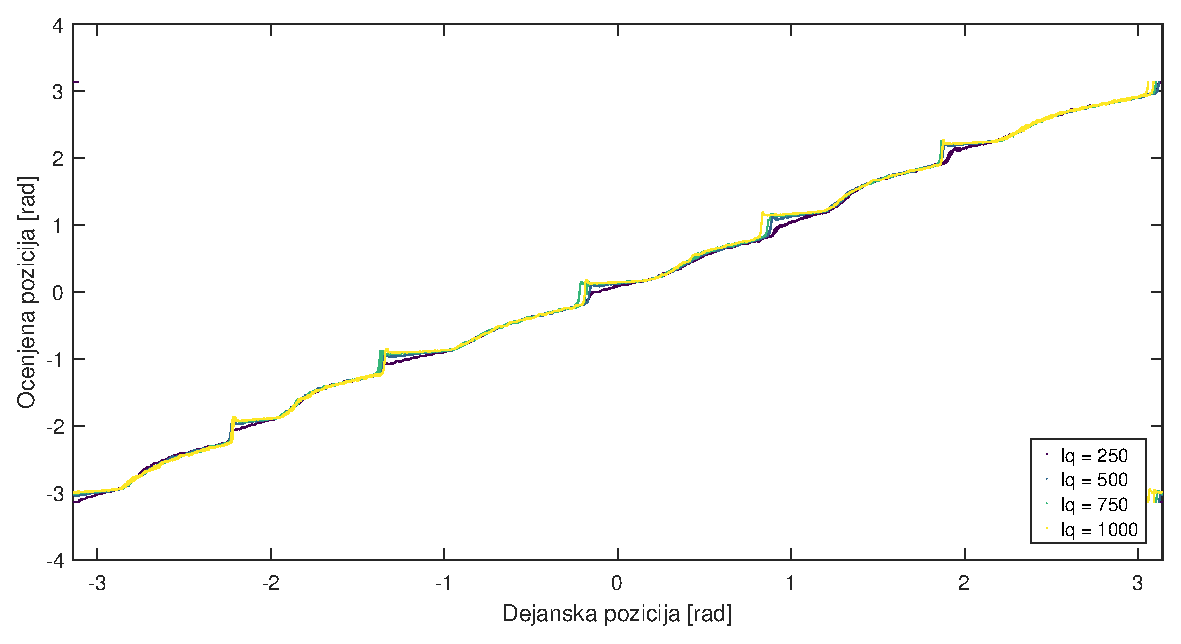
\includegraphics[width=0.9\columnwidth]{Slike/vsiljenaPozicijaMrtviCasPlot_angle.eps}
    \caption{\label{vsiljenaPozicijaMrtviCasPlot_angle} Ocena kota pri različnih mrtvih časih. }
\end{figure}

\begin{figure}[!htbp]
    \centering
    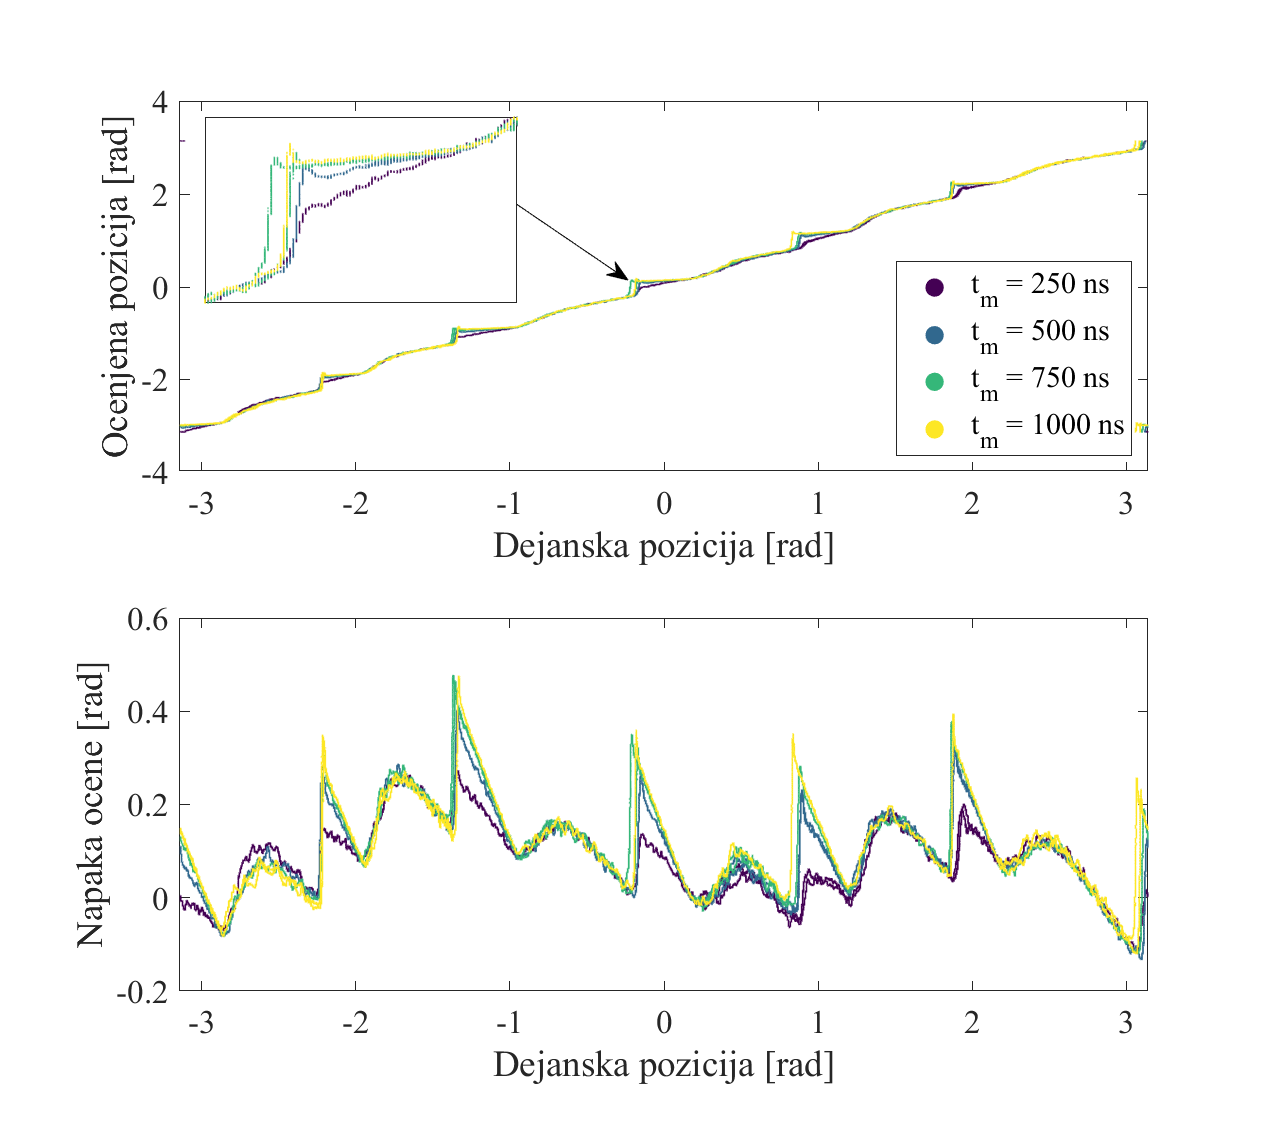
\includegraphics[width=1.05\columnwidth]{Slike/vsiljenaPozicijaMrtviCasPlot_angleError.eps}
    \caption{\label{vsiljenaPozicijaMrtviCasPlot_angleError} Napaka ocene kota pri različnih mrtvih časih. }
\end{figure}

\newpage
Poleg vpliva mrtvega časa se še vedno opazi vpliv višjeharmonskega popačenja, katerega vpliv je bil prikazan na prejšnjih dveh slikah. Smo pa tudi pokazali odvisnost efekta mrtvega časa od faznih
tokov, na slikah \ref{vsiljenaPozicijaMrtviCasPlot_angle} in \ref{vsiljenaPozicijaMrtviCasPlot_angleError} pa se to opazi še na oceni pozicije. Z nižjimi prečnimi tokovi ima večji vpliv mrtvi čas, z
višjimi pa višjeharmonsko popačenje.

% profesor: kako naj poimenujem ta efekt "višjeharmonskega popačenja", če nevem kaj ta efekt povzroča oz od kje to pride in zakaj? Na sestanku sva rekla da je vejetno magnetna asimetrija stroja,
% vendar ne morem temu reči tako, če nisem prepričan da je to res efekt tega. Je vredu da sem poimenoval to tako?

\begin{figure}[!htbp]
    \centering
    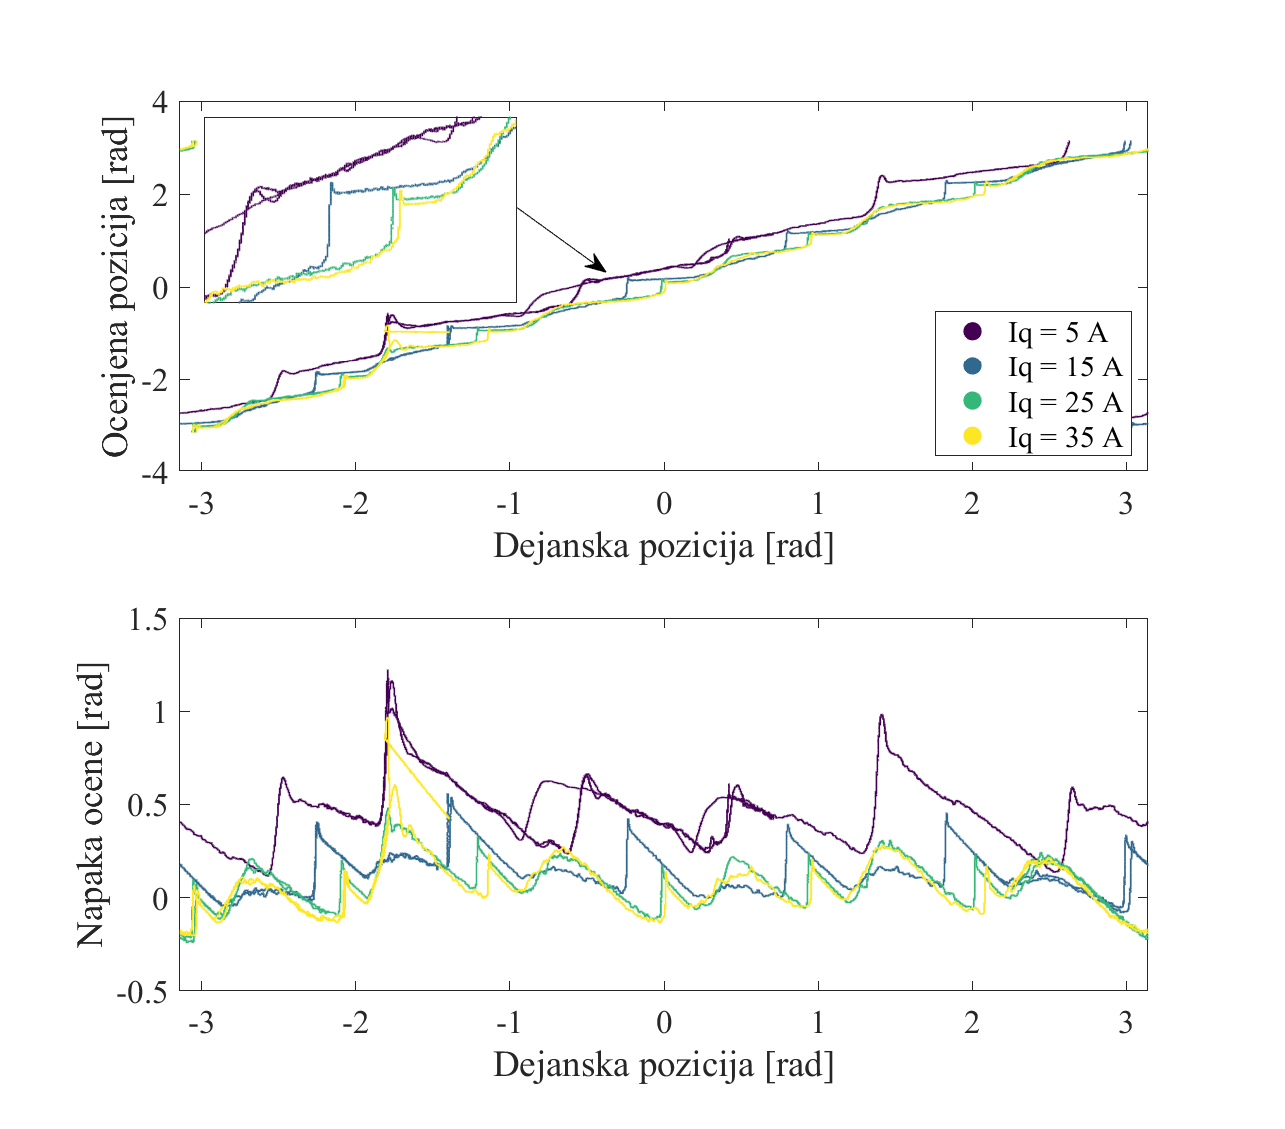
\includegraphics[width=0.9\columnwidth]{Slike/vsiljenaPozicijaTokoviZMrtvimCasom_angle.eps}
    \caption{\label{vsiljenaPozicijaTokoviZMrtvimCasom_angle} Ocena kota pri različnih prečnih tokovih in velikim vrtvim časom. }
\end{figure}

\begin{figure}[!htbp]
    \centering
    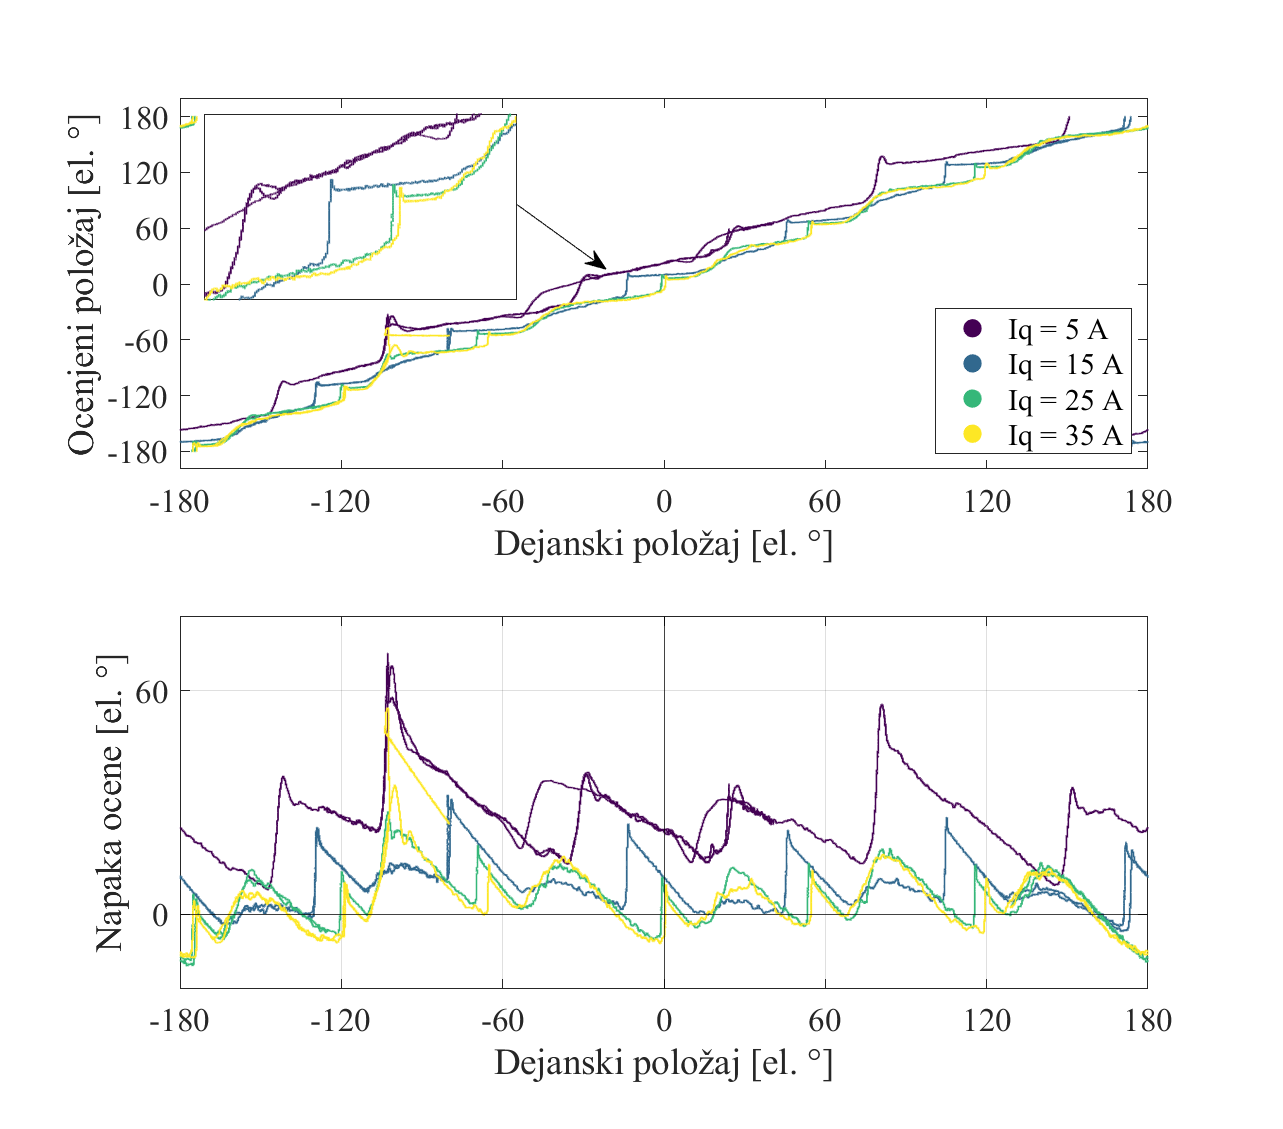
\includegraphics[width=1.05\columnwidth]{Slike/vsiljenaPozicijaTokoviZMrtvimCasom_angleError.eps}
    \caption{\label{vsiljenaPozicijaTokoviZMrtvimCasom_angleError} Napaka ocene kota pri različnih prečnih tokovih in velikim vrtvim časom. }
\end{figure}

Pri tem eksperimentu je bil mrtvi čas $1 \mu s$, kar je v resnici relativno velika vrednost. V praksi je mrtvi čas precej nižji, ne moremo pa se mu izogniti, zato je bil prikazan njegov vpliv.
\\
V prejšnjem poglavju smo omenili izbiro začetne stabilne točke delovanja algoritma in možen vpliv na delovanje. Narejen je bil eksperiment, kjer smo motor počasi vrteli in opazovali ocenjeno pozicijo.
To smo storili za vse štiri začetne točke, kjer je bil prečni tok maksimalen, da se poizkusi delovanje v najslabšem primeru. Na sliki \ref{izbiraStabilneTocke} je prikazana ocena pozicije pri vseh
štirih začetnih točkah, kjer lahko opazimo, da se algoritem obnaša zelo podobno, ne glede na izbiro stabilne pozicije oziroma odklona HKS od RKS:

\begin{figure}[!htbp]
    \centering
    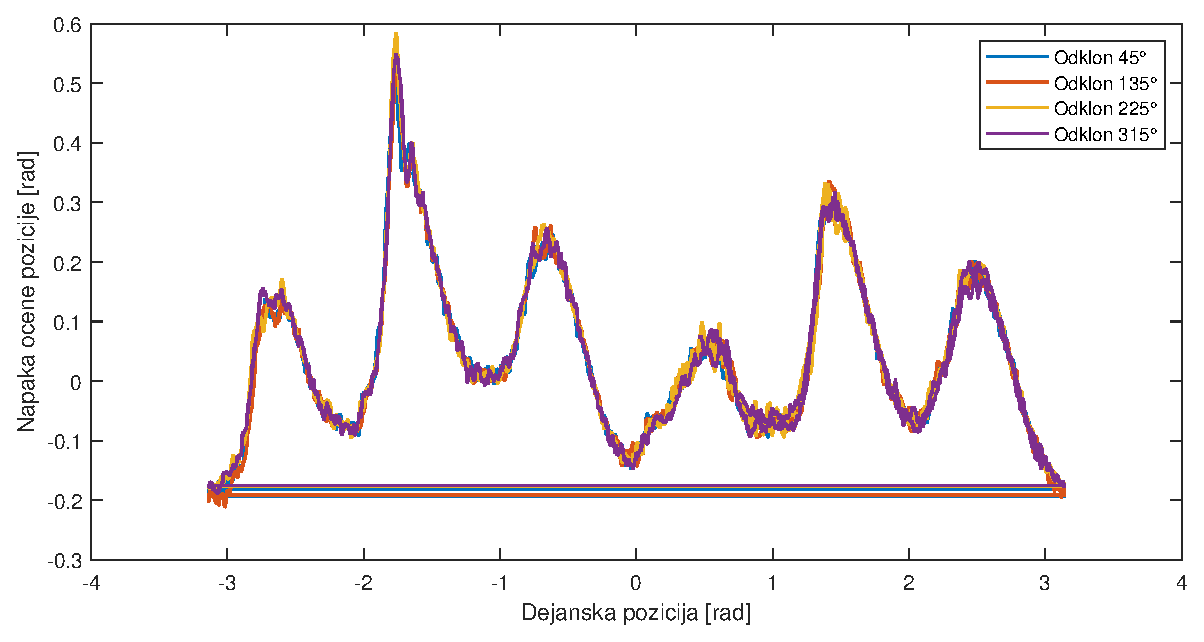
\includegraphics[width=0.75\columnwidth]{Slike/izbiraStabilneTocke.eps}
    \caption{\label{izbiraStabilneTocke} Izbira delovne točke obratovanja regulatorja. }
\end{figure}

%******************************* ZAKLJUČEK *************************************
\chapter{Zaključek} \label{zakljucek}

V sklopu te magistrske neloge smo izdelali algoritem za ocenjevanje pozicije rotorja pri nizkih hitrostih in v nevrtečem stanju. Najprej smo matematično izpeljali pričakovani tokovni odziv kot
posledica vzbujanja in rotorske pozicije. Nato smo pokazali vzbujanje na realnem sistemu in kako ta odstopa od pričakovanega. Dodatno smo pokazali kako mrtvi čas vpliva na tokovni odziv. Opazili smo,
da oceno pozicije najbolj kvari višjeharmonsko popačenje v d-q HKS, katerega nam ni uspelo pojasniti in razrešiti. 

Pokazali smo tudi vpliv enosmernega prečnega toka na delovanje algoritma in opazili, da z višjimi tokovi algoritem deluje slabše, ker se višjeharmonsko popačenje poveča. Pri nižjih tokovih pa se
poveča vpliv mrtvega časa, kar pa lahko mitigiramo z nižanjem le-tega ali nižanjem amplitude vzbujalnega signala.

V primeru nadaljnih raziskav bi bilo smiselno raziskati vir višjeharmonskih popačenj in možne kompenzacije.

%******************************* LITERATURA ************************************
\cleardoublepage\phantomsection\addcontentsline{toc}{chapter}{Literatura} % vnos literature v kazalo

% 1. način: BibTeX
\bibliographystyle{ieeetrslo}
\bibliography{literatura}

% 2. način: neposreden vnos \begin{thebibliography}{99} \bibitem{vir1} C. Su, H. Ke in T. Hubing, ``Overview of Electromagnetic Modeling Software'' [Online], v \textit{25th Annual Review of Progress
%    in Applied Computational Electromagnetics, March 8 - March 12, 2009 - Monterey, California}. Monterey, 2009, str. 736-741. Dosegljivo: \url{http://www.clemson.edu/ces/cvel/pdf/ACES09-736.pdf}.
%    [Dostopano: 23.8.2017]. \bibitem{vir2} T. Hubing et al., ``Survey of Current Computational Electromagnetics Techniques and Software'' [Online]. \textit{Clemson University Vehicular Electronics
%    Laboratory (CVEL)}: Clemson, ZDA, CVEL-08-011.2, 21.9.2008. Dosegljivo: \url{http://www.clemson.edu/ces/cvel/Reports/CVEL-08-011.2.pdf}. [Dostopano: 23.8.2017]. \bibitem{vir3} \textit{The
%    Electromagnetic Radiation Spectrum Poster} [Online]. Dosegljivo: \url{http://www.unihedron.com/projects/spectrum/}. [Dostopano: 23.8.2017]. \end{thebibliography}

%******************************* DODATEK ***************************************
%\appendix

% profesor: dodam tukaj kakšne parametre? Npr frekvenca in amplituda VF signala, PI reg parametri?

\end{document}
%%%%%%%%%%%%%%%%%%%%%%%%%%%%%%%%%%%%%%%%%%%%%%%%%%%%%%%%%%%%%%%%%%%%%%%%%%%%%%%%%%%%%%%%%%%%%%%%%%%%%%%%%%%%%%%%%%%%%%%%
